This section describes the design from the overall architecture down to the individual mechanisms. The whole design follows one rule: the robot must stop whenever any part of the system above the motors fails, and nothing added for the operator or the victim may weaken that guarantee. Sections 3.1 to 3.4 set out the system architecture, the network, the hardware and the software that runs on it. Sections 3.5 to 3.7 then follow the stop guarantee upward through the tiers: the firmware enforces it (3.5), the control server feeds it safely (3.6), and supervision restores service after a failure without bypassing it (3.7). Section 3.8 decides which operator holds control, and Section 3.9 builds victim interaction on that decision while keeping it apart from the stop path. Section 3.10 adds localisation for the operator.

\section*{3.0 Design Rationale and Relation to Research Questions}
\addcontentsline{toc}{section}{3.0 Design Rationale and Relation to Research Questions}

This chapter describes the system design: the structure, mechanisms and design choices that realise the stop guarantee stated above. The procedures and metrics that validate the design belong to Section 4 (Experimental Setup) and the measurements to Section 5 (Results); this chapter does not repeat them, but cross-references the relevant Section 4 and Section 5 subsection, and the raw data under \texttt{tools/eval/}, at each point where a design choice has an empirical test. Each design pillar below is traced to the research question that motivates it and to the Section 5 subsection that evaluates it, with the state of that evidence. The research questions RQ1 to RQ4 are stated in Section 1.3; RQ4 covers both the two-way victim path and GPS and mapping.

\begin{itemize}
\item Firmware dead-man and ramp-stop (Section 3.5.2) $\rightarrow$ RQ1 $\rightarrow$ Section 5.1: the firmware-side stop interval is measured from logs (Table 5.2b); the physical wheel-stop time (E4) is [PENDING MEASUREMENT]; the heartbeat-loss margin (Section 5.1b) is SIMULATED
\item P1 single-writer serial link and session resume (Section 3.6) $\rightarrow$ RQ2 $\rightarrow$ Sections 5.1 and 5.3: control-plane latency is a robot-internal upper bound with no Wi-Fi figure, the range sweep is partial, and session resume was not measured
\item P3 process isolation and supervision (Section 3.7) $\rightarrow$ RQ3 $\rightarrow$ Section 5.4: automated SIGKILL recovery, 30 of 30 trials, plus single manual injections
\item WebRTC two-way victim path (Section 3.9) $\rightarrow$ RQ4 $\rightarrow$ Section 5.5 for the measured processor cost and isolation of the media process; video and audio delay and quality (Section 5.2, E5) and the end-to-end rescue run (Section 5.7, E13) are [PENDING MEASUREMENT]
\item GPS and offline map (Section 3.10) $\rightarrow$ RQ4 $\rightarrow$ Section 5.6.1: static precision is measured but resolution-limited, and the 10 m track filter admitted drift
\end{itemize}

\section{System Architecture}

The architecture applies the design rule by separating the system into tiers that can fail on their own, each failure ending at the firmware stop. The system has four tiers: an Arduino UNO for real-time control, a Raspberry Pi 4, a local Wi-Fi network, and a browser dashboard (Figure 1). The Pi runs three separate Python processes: P1 (control server) links the dashboard to the Arduino, checks every drive command and collects telemetry and GPS; P2 (media server) streams the robot's camera and microphone to the operator and carries the operator's voice, video and text to the robot's screen; and P3 (watchdog) starts P1 and P2 and restarts either one if it crashes or stops responding. Control and media use separate transports that end in separate processes, so a media failure leaves driving and stopping intact.

\begin{diagramfig}
\makebox[\textwidth][c]{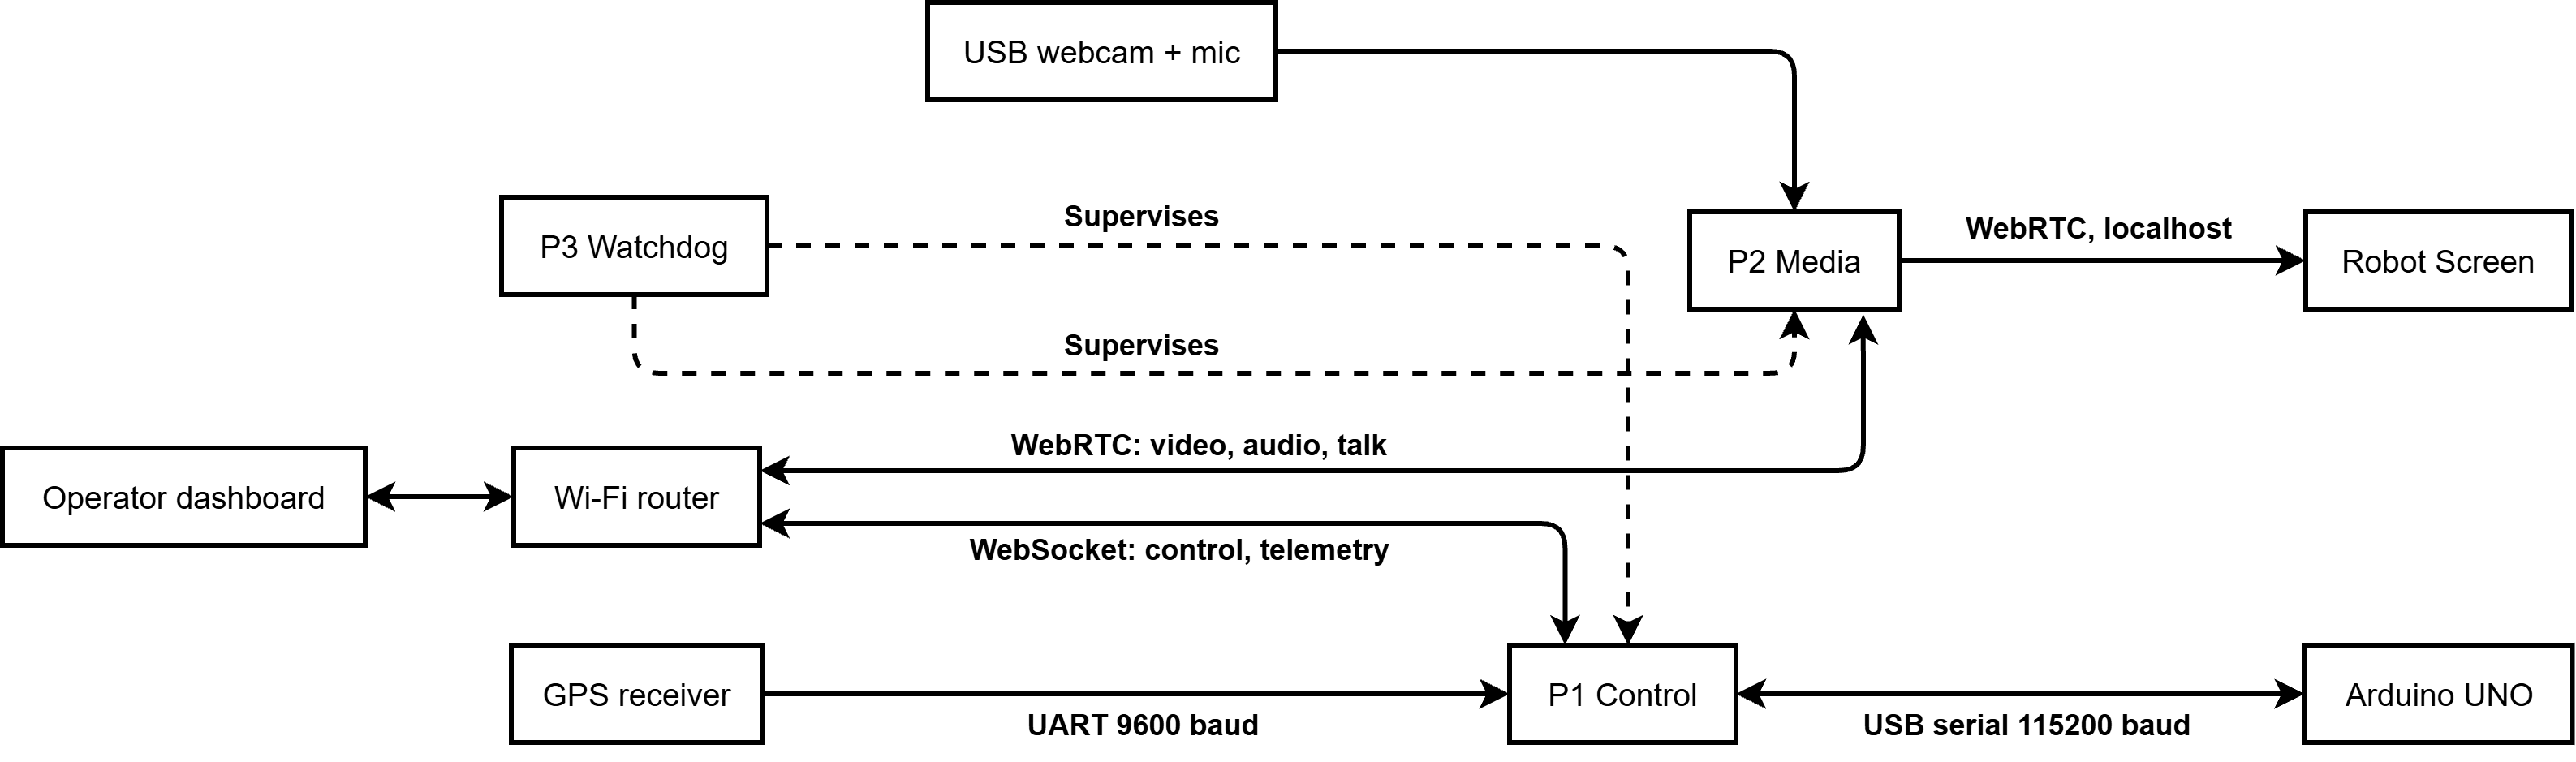
\includegraphics[width=1.15\textwidth]{fig01.png}}
\caption{Overall system architecture.}
\end{diagramfig}

Figure 2 follows one drive command through every tier and the telemetry that returns. A held key sends one motion command; while it is held, heartbeats keep the dead-man armed, and releasing the key sends a stop.

\clearpage
\begin{figure}[H]
\centering\footnotesize
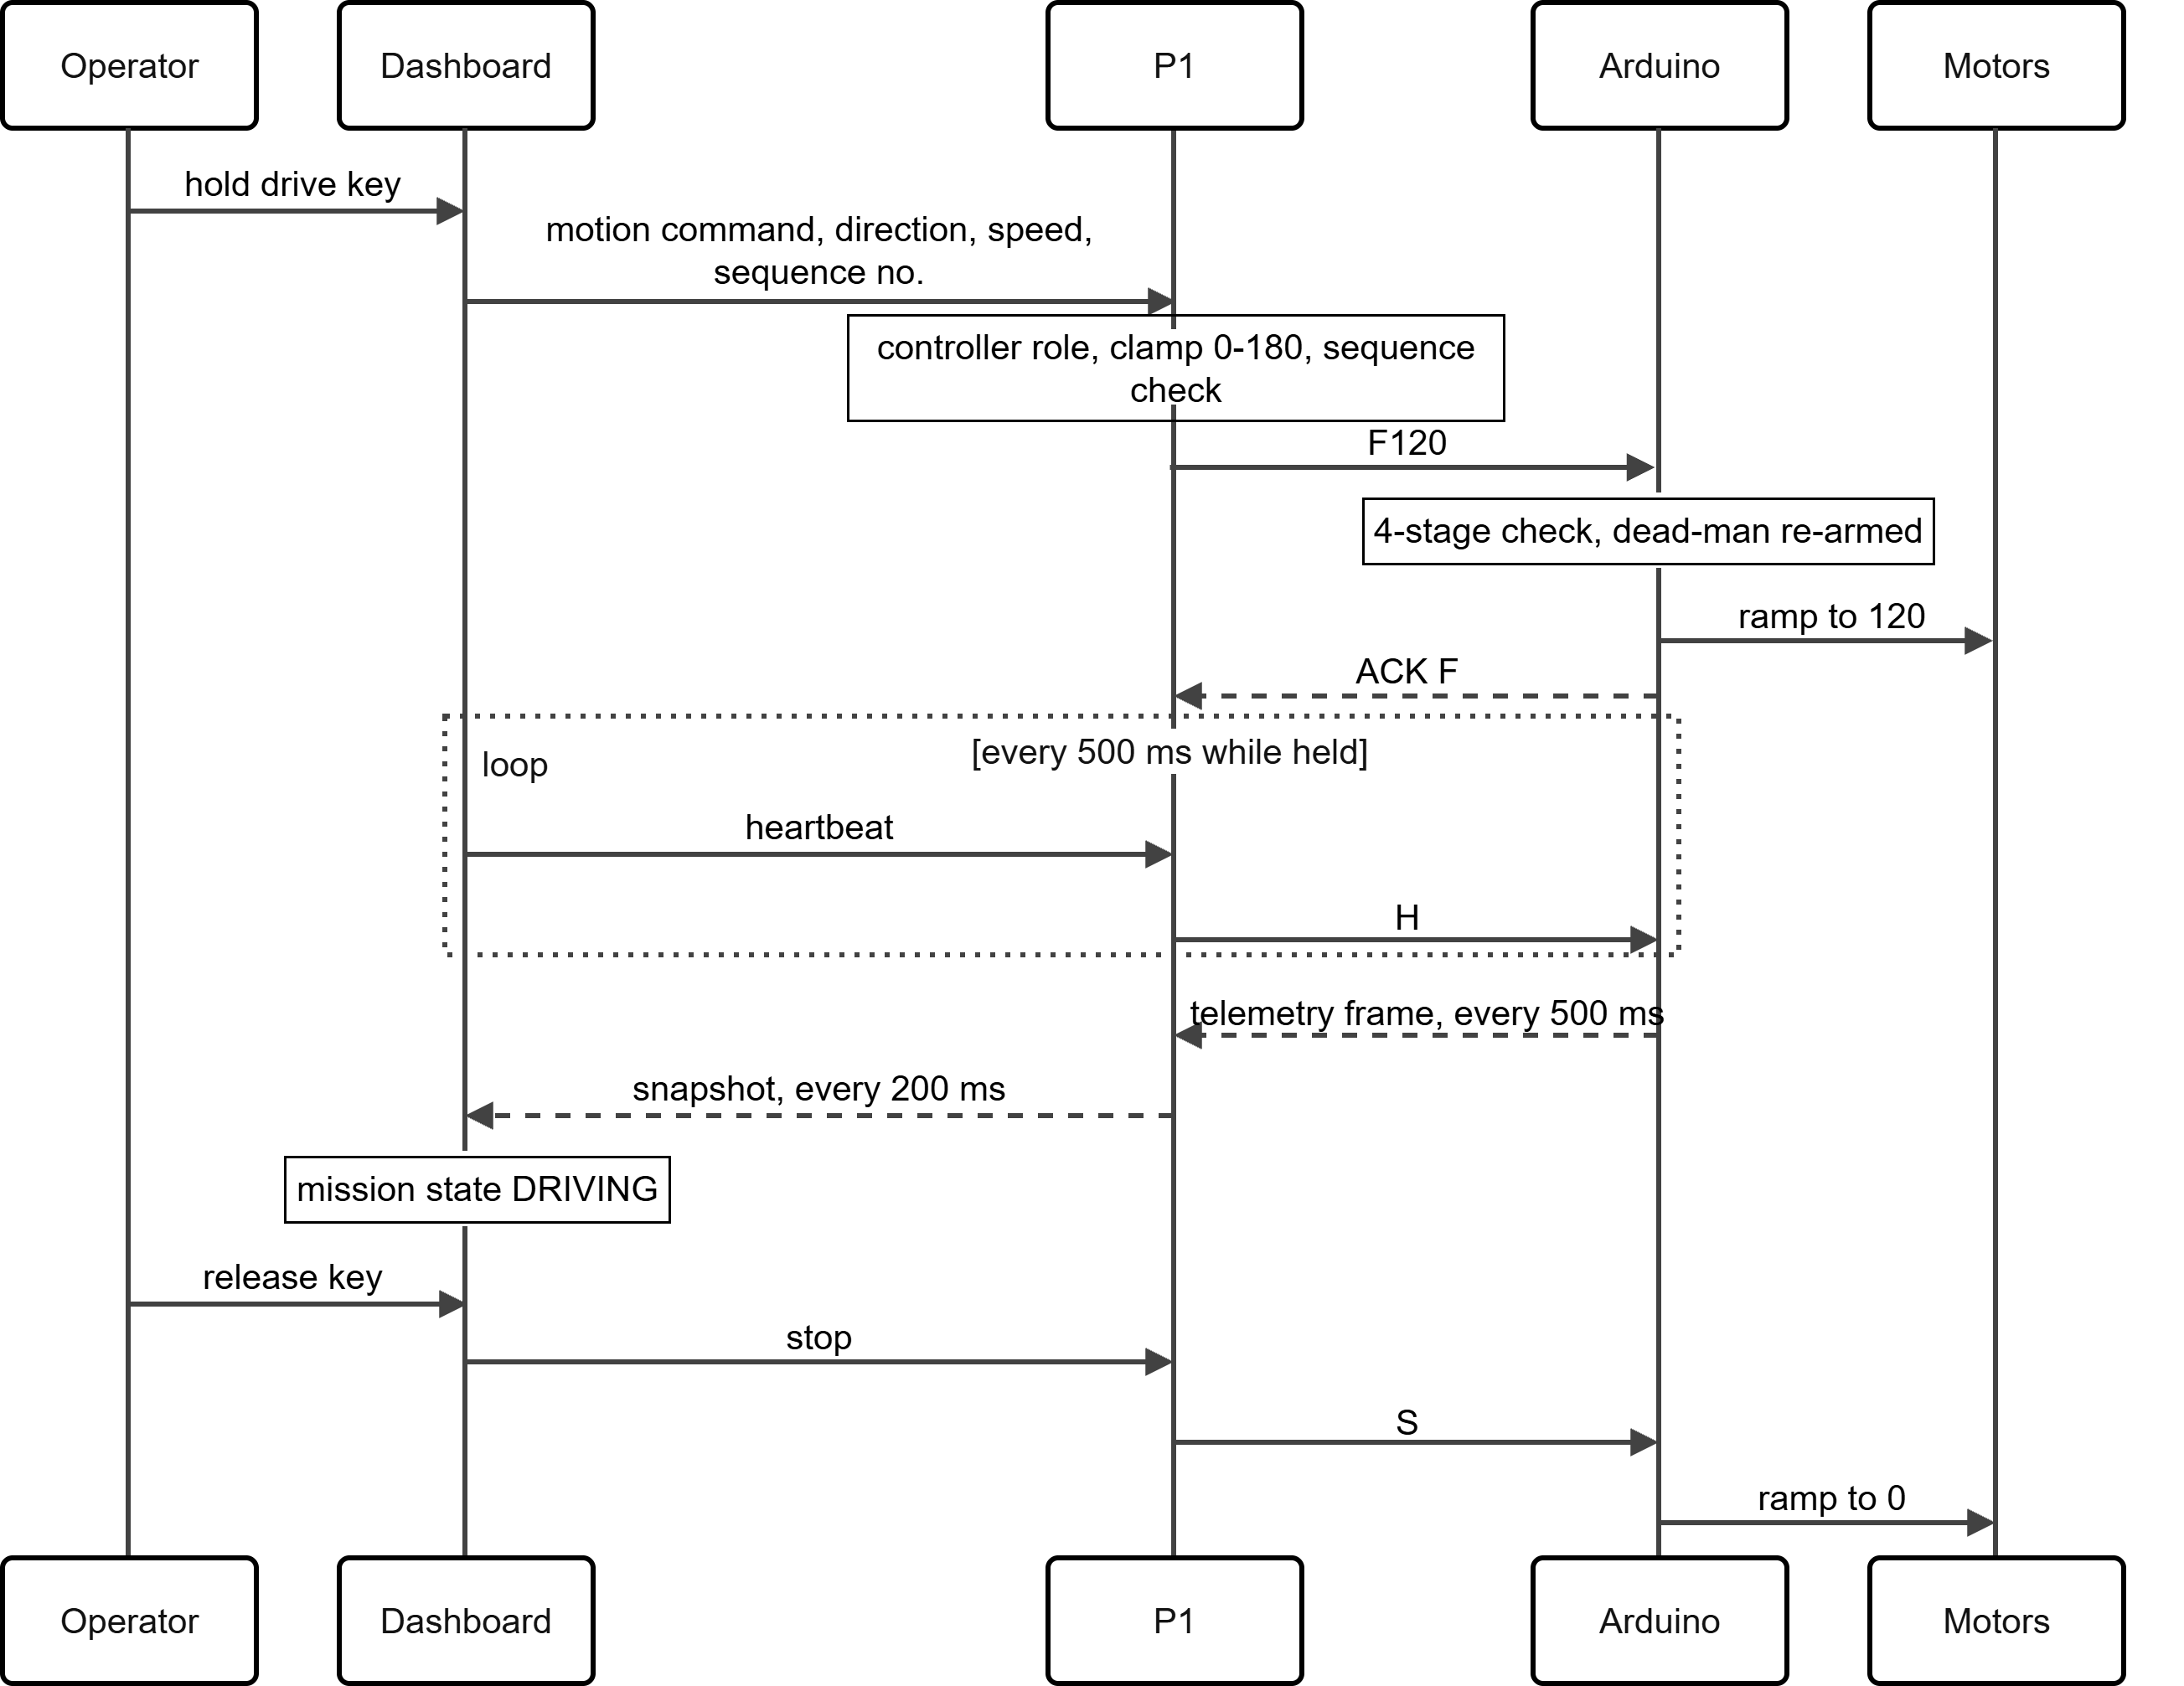
\includegraphics[width=\textwidth]{fig02.png}
\caption{End-to-end control loop: command down, telemetry up.}
\end{figure}

P2 and P3 take no part in this loop: media never carries a drive or stop command, and the watchdog only supervises the processes from outside, so a failure in either cannot delay a stop.

\section{Network Configuration}

The two transports in Figure 1 run over one local network, which also makes the robot independent of the internet: no part of the deployment evaluated here reaches outside the Wi-Fi cell. The Pi and the operator laptop join the existing Wi-Fi network, an 802.11n cell on the 2.4 GHz band on channel 10 (2457 MHz) with a 20 MHz operating width (the access point was on channel 3 for two stations on 2026-10-22; Section 5.3). Both hold addresses in the same /24 subnet, so traffic between them is neither routed nor address-translated, which is what lets the media path of Section 3.9.2 rely on host candidates alone. The Pi uses its on-board radio (Figure 5) and takes its address from the router by DHCP: in the deployment measured here it held 192.168.0.105 in 192.168.0.0/24 with the router at 192.168.0.1, on a lease rather than a reservation, so the operator reads the current address off the Pi (\texttt{ip addr show wlan0}) before opening the dashboard. The project supplies no network configuration of its own, neither an access point nor a DHCP reservation nor a static address, so the subnet is whatever the router hands out. The router stays with the operator at the staging point, so the robot works within one radio cell, and extending that reach with a repeater or a second radio is outside the scope of this work (Section 6.3). Table~\ref{tab:network-services} lists the services on the Pi and Table~\ref{tab:network-load} the load and the timing the network has to carry.

\begin{center}
\begin{longtable}{|l|l|l|p{6cm}|}
\caption{Network services on the Pi.}
\label{tab:network-services} \\
\hline
\textbf{Port} & \textbf{Process} & \textbf{Protocol} & \textbf{Carries} \\
\hline
\endfirsthead
\hline
\textbf{Port} & \textbf{Process} & \textbf{Protocol} & \textbf{Carries} \\
\hline
\endhead
TCP 8080 & P1 & HTTP and WebSocket & Dashboard files, control and telemetry, session settings, GPS track, offline map tiles, ICE configuration (Section 3.9.2), health \\
\hline
TCP 8443 & P2 & HTTP (no TLS) & WebRTC offer and answer, Robot Screen page, health \\
\hline
UDP, negotiated by ICE & P2 & WebRTC & Audio, video and data channel \\
\hline
Localhost only & P1, P2 & HTTP & Controller address query; Robot Screen connection \\
\hline
\end{longtable}
\end{center}

Control and media use different transports for different reasons. Commands and telemetry run over TCP, because ordered delivery together with the sequence check of Section 3.5.1 keeps a stale command from overtaking a newer one, and the cost of a retransmission is bounded: a command that does not arrive within the dead-man window stops the robot instead of leaving it to run on a stale one (Section 3.5.2). Media runs over UDP, where a lost packet costs picture or voice quality but never delays a command. The dead-man window therefore sets the only hard requirement the network must meet, and the budgets in Table~\ref{tab:network-load} follow from it.

\begin{center}
\begin{longtable}{|p{5cm}|p{4cm}|p{4cm}|}
\caption{Network load and timing requirements.}
\label{tab:network-load} \\
\hline
\textbf{Quantity} & \textbf{Value} & \textbf{Set by} \\
\hline
\endfirsthead
\hline
\textbf{Quantity} & \textbf{Value} & \textbf{Set by} \\
\hline
\endhead
Video, robot to operator & 640x480 at 10 fps, 500 kbps target & Section 3.9.1, Table~\ref{tab:video-parameters} \\
\hline
Audio, each direction & Opus 32 kbps, 60 ms packets & Table~\ref{tab:audio-parameters} \\
\hline
Telemetry snapshots & 5 per second from P1, one JSON object each; the firmware frames behind them arrive every 500 ms & Section 3.6.2 \\
\hline
Commands and heartbeats & Heartbeat every 500 ms from the controller; one drive command per press and per release; servo commands are not rate limited & Sections 3.5.1 and 3.6 \\
\hline
Steady-state load per operator & Under 1 Mbit/s & Sum of the rows above \\
\hline
Hard delivery deadline & 2000 ms since the last arming command & Dead-man, Section 3.5.2 \\
\hline
Operator-side link timeout & 3000 ms without telemetry gives mission state STOP, counted in 500 ms steps & Table~\ref{tab:mission-state} \\
\hline
Socket keep-alive & Ping every 20 s, 20 s timeout & P1 WebSocket server \\
\hline
Reconnect back-off & 1 s, doubling, capped at 30 s & Section 3.7.2 \\
\hline
\end{longtable}
\end{center}

Four intervals bear on the dead-man window, and none of them is a count of the others. The dashboard sends a heartbeat every 500 ms for as long as it holds the controller role, whether or not the robot is being driven; a drive command is sent once when a key or button goes down and a stop once when it is released, with keyboard auto-repeat suppressed, so a sustained drive is carried by the heartbeat rather than by repeated commands. The firmware re-arms its dead-man timer on any arming command it accepts, heartbeats included, and stops the motors once 2000 ms pass with none: an absolute window measured from the last accepted command, not a threshold of missed heartbeats. Independently of that window the firmware emits a telemetry frame every 500 ms and a compact heartbeat line every 1000 ms, but both are outbound reports and neither re-arms the timer. A 2000 ms window spans four heartbeat periods at the configured 500 ms rate, so an occasional lost heartbeat does not stop the robot: two consecutive losses leave a gap of 1500 ms, and a third reaches the window. The dashboard did not always keep that rate; at the 1 s period logged in some sessions, a single lost heartbeat already reaches the window (Section 5.4, Table 5.9d).

The load stays well inside the capacity of an ordinary indoor Wi-Fi link: at the staging point the link negotiated 58.5 Mbit/s receive and 72.2 Mbit/s transmit at a signal level of about -47 dBm, more than fifty times the steady-state demand, so the network is sized by latency and loss rather than by throughput, and Section 5.3 reports how both varied over the distances tested; the dashboard bundle and the offline map tiles are one-off transfers at the start of a session. The keep-alive in Table~\ref{tab:network-load} reclaims a silently dead socket only after up to 40 s, so liveness for safety is not enforced at this layer but by the dead-man at 2000 ms and by the dashboard's 3000 ms telemetry timeout; the keep-alive only frees the socket. Browsers allow microphone and camera capture only in a secure context, and neither port carries TLS (Table~\ref{tab:network-services}), so the operator's browser has to be told to treat the Pi's origin as trusted, through the insecure-origin exception recorded in the operator manual. Push-to-talk and the operator camera depend on that manual step, which is a deployment workaround rather than a configured transport security measure (Section 6.3); images and text work without it.

\section{Hardware Platform}

The hardware is chosen so that the lowest tier can stop the robot by itself: the Arduino drives the motor drivers directly and can disable them with one output. Table~\ref{tab:hardware-components} lists the components, and Figure 3 shows how they connect and how power is distributed. The motor supply and the Pi supply are separate, so motor current surges cannot reset the Pi.

\begin{center}
\begin{longtable}{|p{3.5cm}|p{4.5cm}|p{5.5cm}|}
\caption{Hardware components.}
\label{tab:hardware-components} \\
\hline
\textbf{Component} & \textbf{Part} & \textbf{Function} \\
\hline
\endfirsthead
\hline
\textbf{Component} & \textbf{Part} & \textbf{Function} \\
\hline
\endhead
Edge computer & Raspberry Pi 4 Model B, 4 GB & Runs P1, P2, P3 and the Robot Screen \\
\hline
Microcontroller & Arduino UNO (ATmega328P, 16 MHz) & Real-time control and sensing \\
\hline
Motor drivers & 2 x BTS7960 & One driver per side \\
\hline
Drive motors & 4 x 25GA-370 geared DC motor with encoder, 12 V, 60 RPM no-load, 65 mm wheels & Differential (skid) steering, left and right pairs \\
\hline
Camera servos & 2 x TowerPro SG90 micro servo, about 1.8 kgf-cm stall torque at 4.8 V, 180 deg & Pan and tilt, 0-180 deg, home at 90 deg \\
\hline
Range sensor & HC-SR04 & Forward range, 0-400 cm \\
\hline
Temperature and humidity & DHT11 & degC and \% RH \\
\hline
Gas sensor & MQ-136 & Raw 10-bit value 0-1023, uncalibrated \\
\hline
GPS receiver & NEO-6M & Position, fix, satellite count \\
\hline
Camera and microphone & USB webcam with built-in microphone & 640x480 video at 10 fps; 48 kHz audio \\
\hline
Robot display & 7-inch HDMI display, 1024x600 & Victim-facing Robot Screen \\
\hline
Speaker & Speaker & Operator voice to the victim \\
\hline
Battery & 4S3P Li-ion pack (twelve 18650 cells, 1500 mAh each), 14.8 V nominal, 16.8 V full, 4.5 Ah nominal, continuous discharge limited by the 4S 40 A BMS & Motor and logic power \\
\hline
Battery management & 4S 40 A BMS & Pack protection \\
\hline
Buck converters & 2 x buck converter, 8 V and 5 V outputs & 8 V to the Arduino barrel jack; 5 V to the servos \\
\hline
Pi supply & Remax 50000 mAh USB power bank & Separate supply for the Pi \\
\hline
\end{longtable}
\end{center}

\clearpage
\begin{figure}[H]
\centering\footnotesize
\makebox[\textwidth][c]{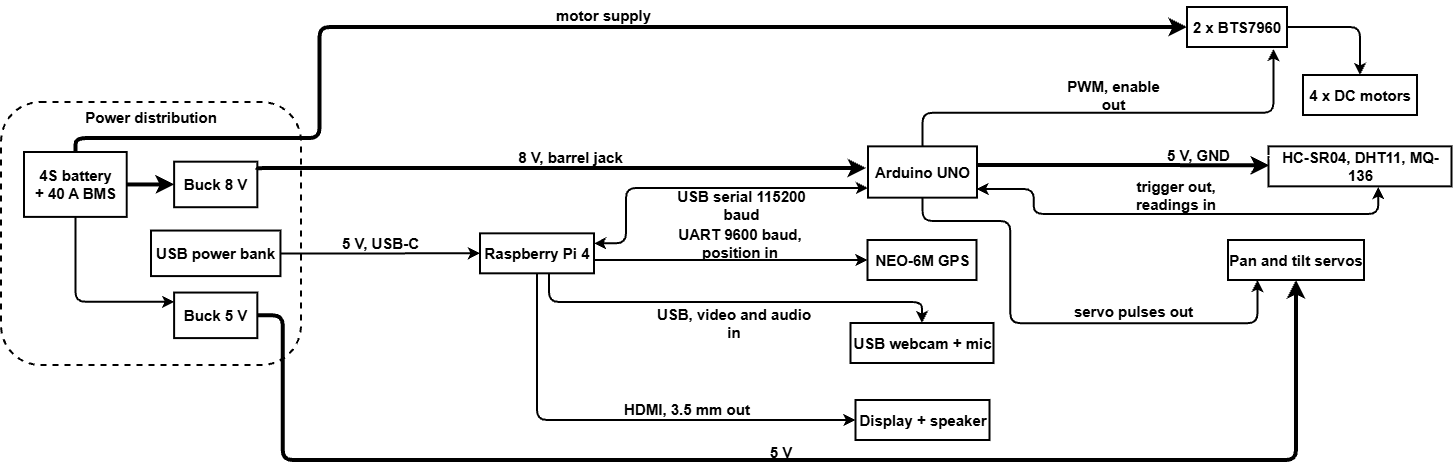
\includegraphics[width=1.22\textwidth]{fig03.png}}
\caption{Hardware interconnection and power distribution. Thick lines carry power; thin lines carry signals, labelled with the interface and its direction. The Pi and the Arduino are the two hubs, and the separate motor and Pi supplies are grouped on the left.}
\end{figure}

The Arduino pins used by the firmware are shown in Figure 4 and detailed in Table~\ref{tab:arduino-pin-map}. Each BTS7960 drives forward on one PWM input and reverse on the other, with only one active at a time; both drivers share one enable line, so one output disables all propulsion.

\begin{figure}[H]
\centering\footnotesize
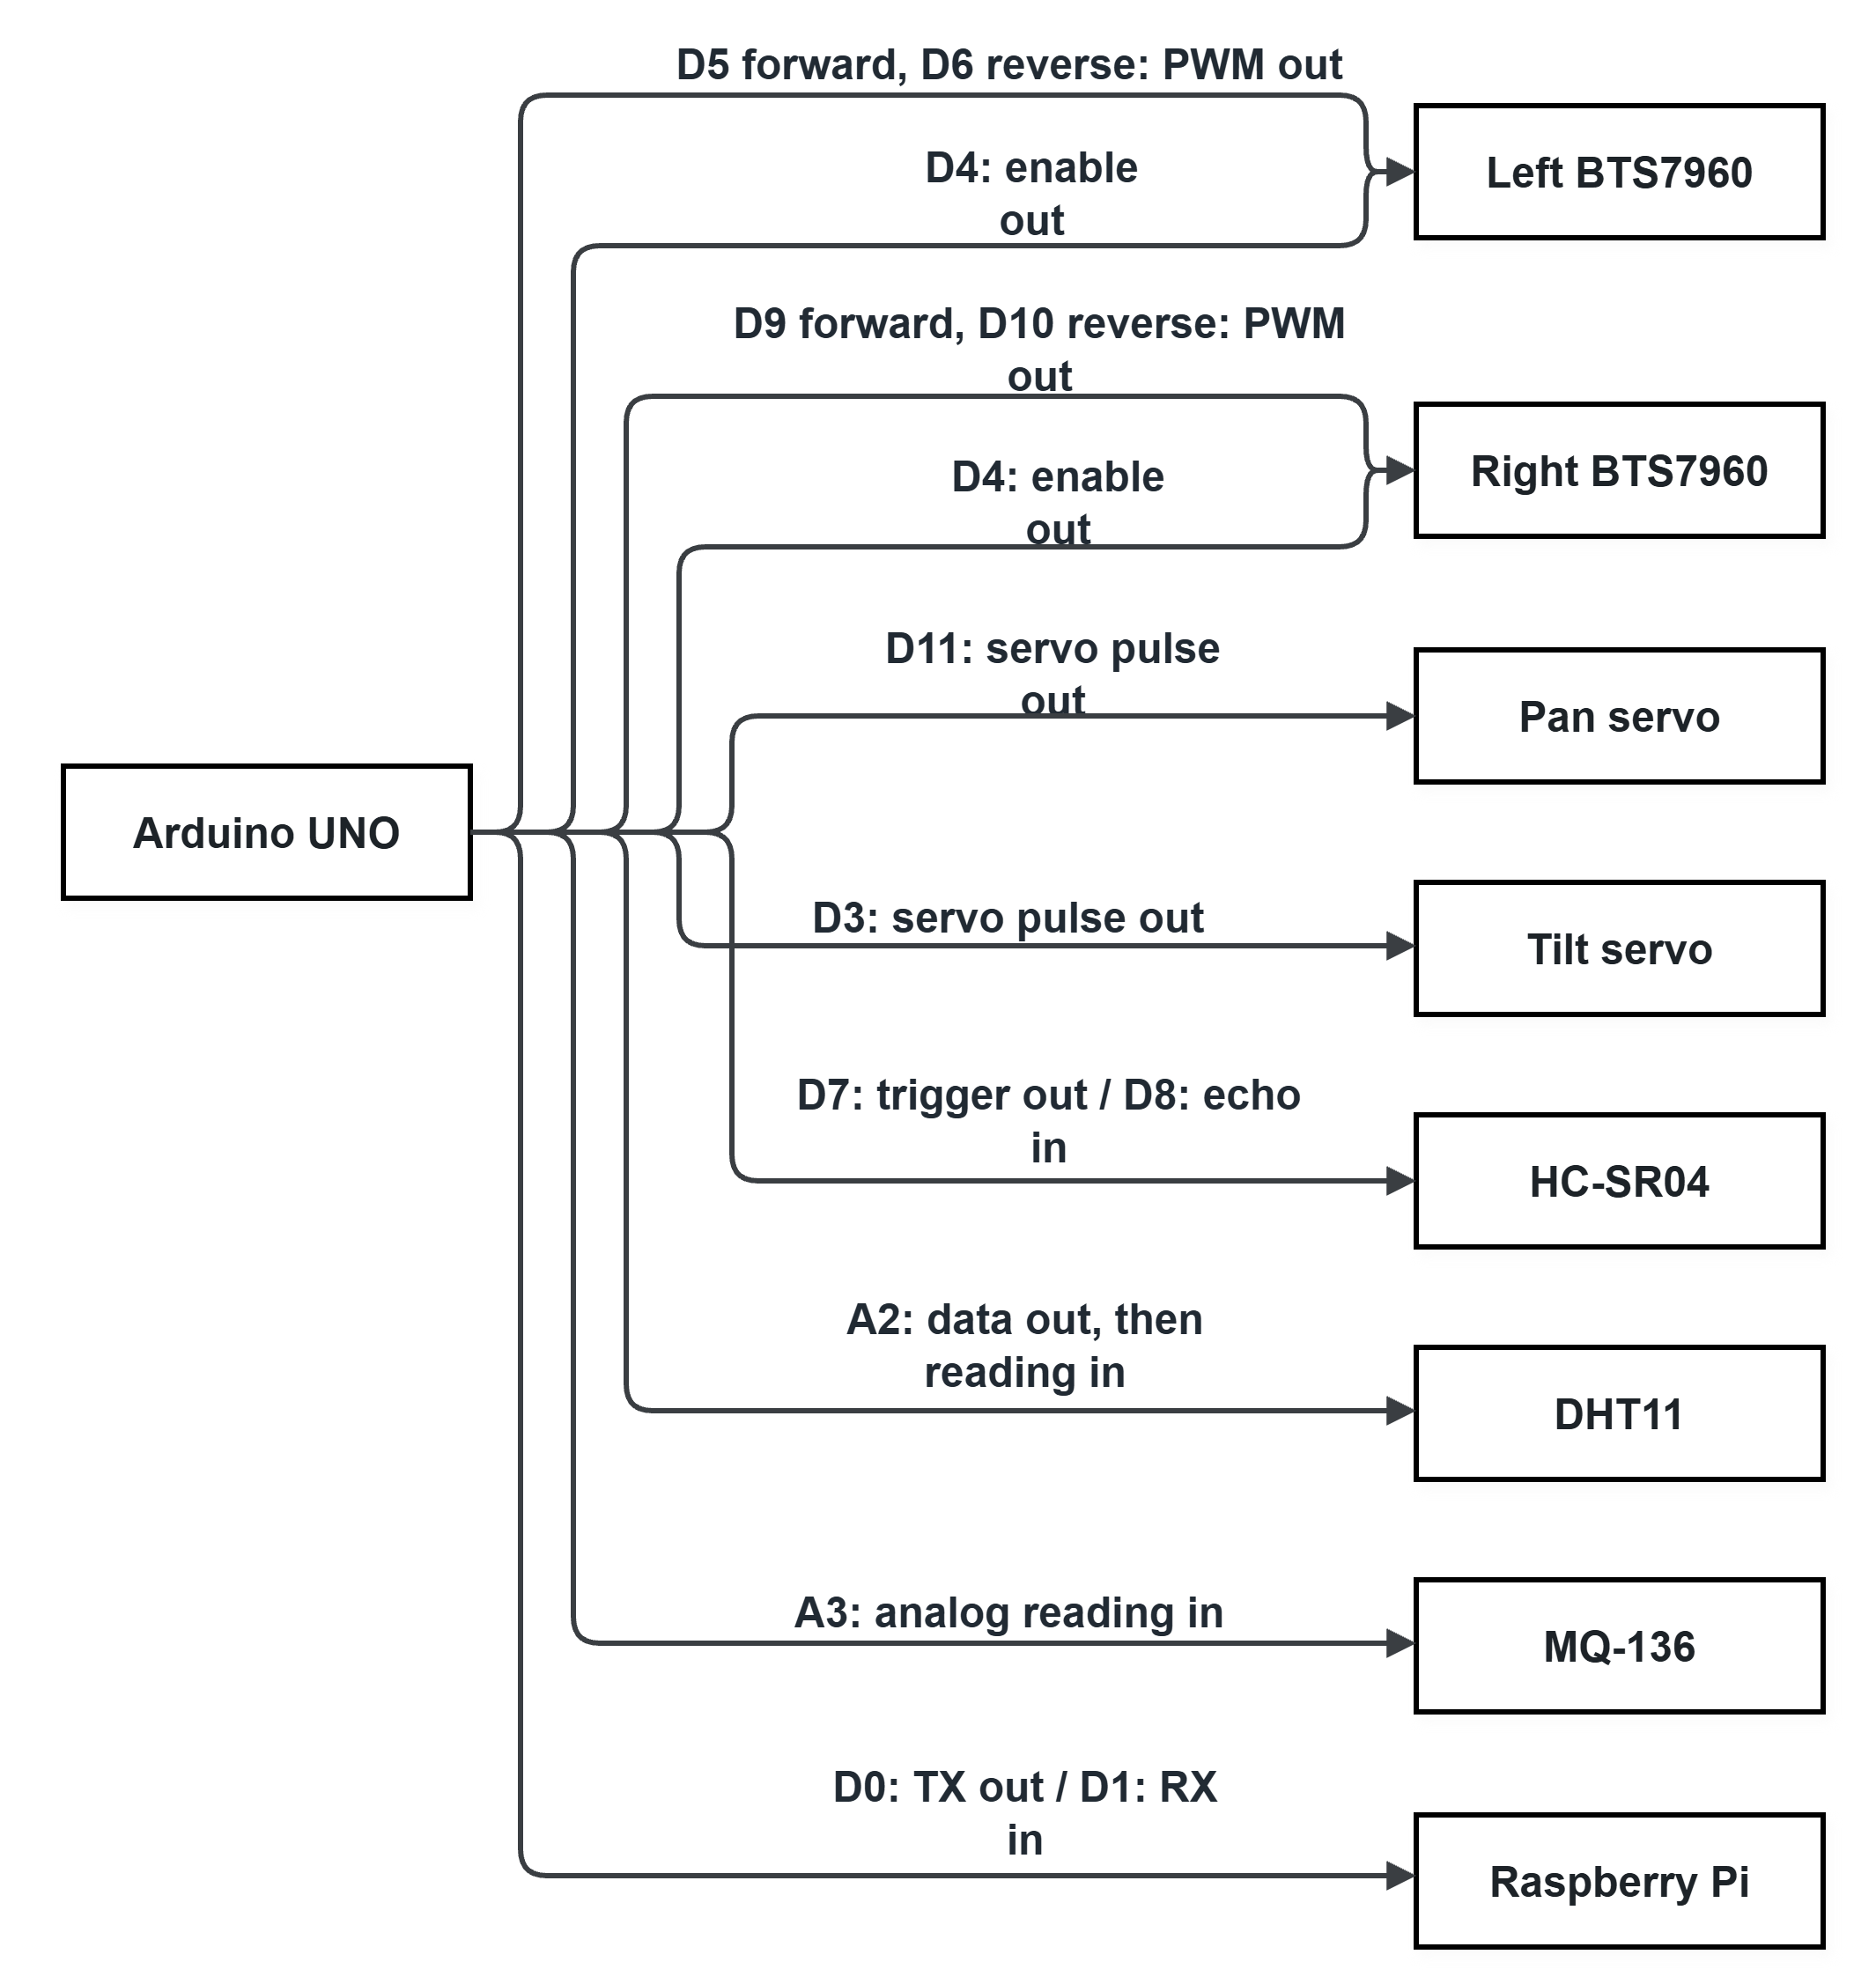
\includegraphics[height=11.8cm,keepaspectratio]{fig04.png}
\end{figure}

\clearpage
\begin{figure}[H]
\centering\footnotesize
\caption{Arduino UNO pin diagram. Every line is drawn from the Arduino outwards to the device it serves, so an arrowhead marks the connection and not the signal direction. Direction is given in the label instead, read from the Arduino's side: "out" leaves the pin and "in" arrives at it, and a label with both names the outgoing pin first. Table~\ref{tab:arduino-pin-map} gives the full pin map.}
\end{figure}

\begin{center}
\begin{longtable}{|l|l|p{3.5cm}|p{4.5cm}|}
\caption{Arduino UNO pin map.}
\label{tab:arduino-pin-map} \\
\hline
\textbf{Pin} & \textbf{Mode} & \textbf{Signal} & \textbf{Notes} \\
\hline
\endfirsthead
\hline
\textbf{Pin} & \textbf{Mode} & \textbf{Signal} & \textbf{Notes} \\
\hline
\endhead
D0, D1 & UART over USB & Serial link to the Pi & 115200 baud, newline-terminated ASCII \\
\hline
D3 & Output & Tilt servo pulse & ServoTimer2Plus library on Timer2, 0-180 deg \\
\hline
D4 & Digital output & Enable for both BTS7960 drivers & Low at boot and on emergency stop \\
\hline
D5 & PWM output & Left driver, forward & 0-255 \\
\hline
D6 & PWM output & Left driver, reverse & 0-255 \\
\hline
D7 & Digital output & HC-SR04 trigger & 10 us pulse every 50 ms \\
\hline
D8 & Digital input & HC-SR04 echo & 25 ms timeout; distance = pulse width / 58 \\
\hline
D9 & PWM output & Right driver, forward & 0-255; Timer1 left free for these pins \\
\hline
D10 & PWM output & Right driver, reverse & 0-255 \\
\hline
D11 & Output & Pan servo pulse & ServoTimer2Plus library on Timer2, 0-180 deg \\
\hline
D13 & Digital output & On-board status LED & Toggles every 1000 ms \\
\hline
A2 & Digital I/O, pull-up & DHT11 single-wire data & Read every 2000 ms, checksum verified \\
\hline
A3 & Analog input & MQ-136 output & 10-bit ADC; raw value reported in telemetry \\
\hline
Barrel jack & Power input & 8 V from buck converter & - \\
\hline
5 V, GND & Power output & Supply for HC-SR04, DHT11 and MQ-136 & Shared by the three sensors \\
\hline
\end{longtable}
\end{center}

\begin{center}
\begin{longtable}{|p{3.5cm}|p{4cm}|p{5cm}|}
\caption{Raspberry Pi 4 connections.}
\label{tab:pi-connections} \\
\hline
\textbf{Pi interface} & \textbf{Connected to} & \textbf{Use} \\
\hline
\endfirsthead
\hline
\textbf{Pi interface} & \textbf{Connected to} & \textbf{Use} \\
\hline
\endhead
USB-A & Arduino UNO & USB serial, 115200 baud \\
\hline
USB-A & USB webcam with microphone & Video capture and audio capture \\
\hline
Header pin 1 (3.3 V) & GPS VCC & GPS supply \\
\hline
Header pin 6 (GND) & GPS GND & Ground \\
\hline
Header pin 8 (GPIO 14, TXD) & GPS RX & UART, 9600 baud \\
\hline
Header pin 10 (GPIO 15, RXD) & GPS TX & UART, 9600 baud \\
\hline
Micro-HDMI 0 & Robot display & Robot Screen \\
\hline
3.5 mm jack & Speaker & Default audio output \\
\hline
USB-C & USB power bank & Pi supply \\
\hline
On-board Wi-Fi & Wi-Fi router & Dashboard, control and media traffic \\
\hline
\end{longtable}
\end{center}

The Pi ports and GPIO header pins used by the project are shown in Figure 5 and listed in Table~\ref{tab:pi-connections}.

\begin{figure}[H]
\centering\footnotesize
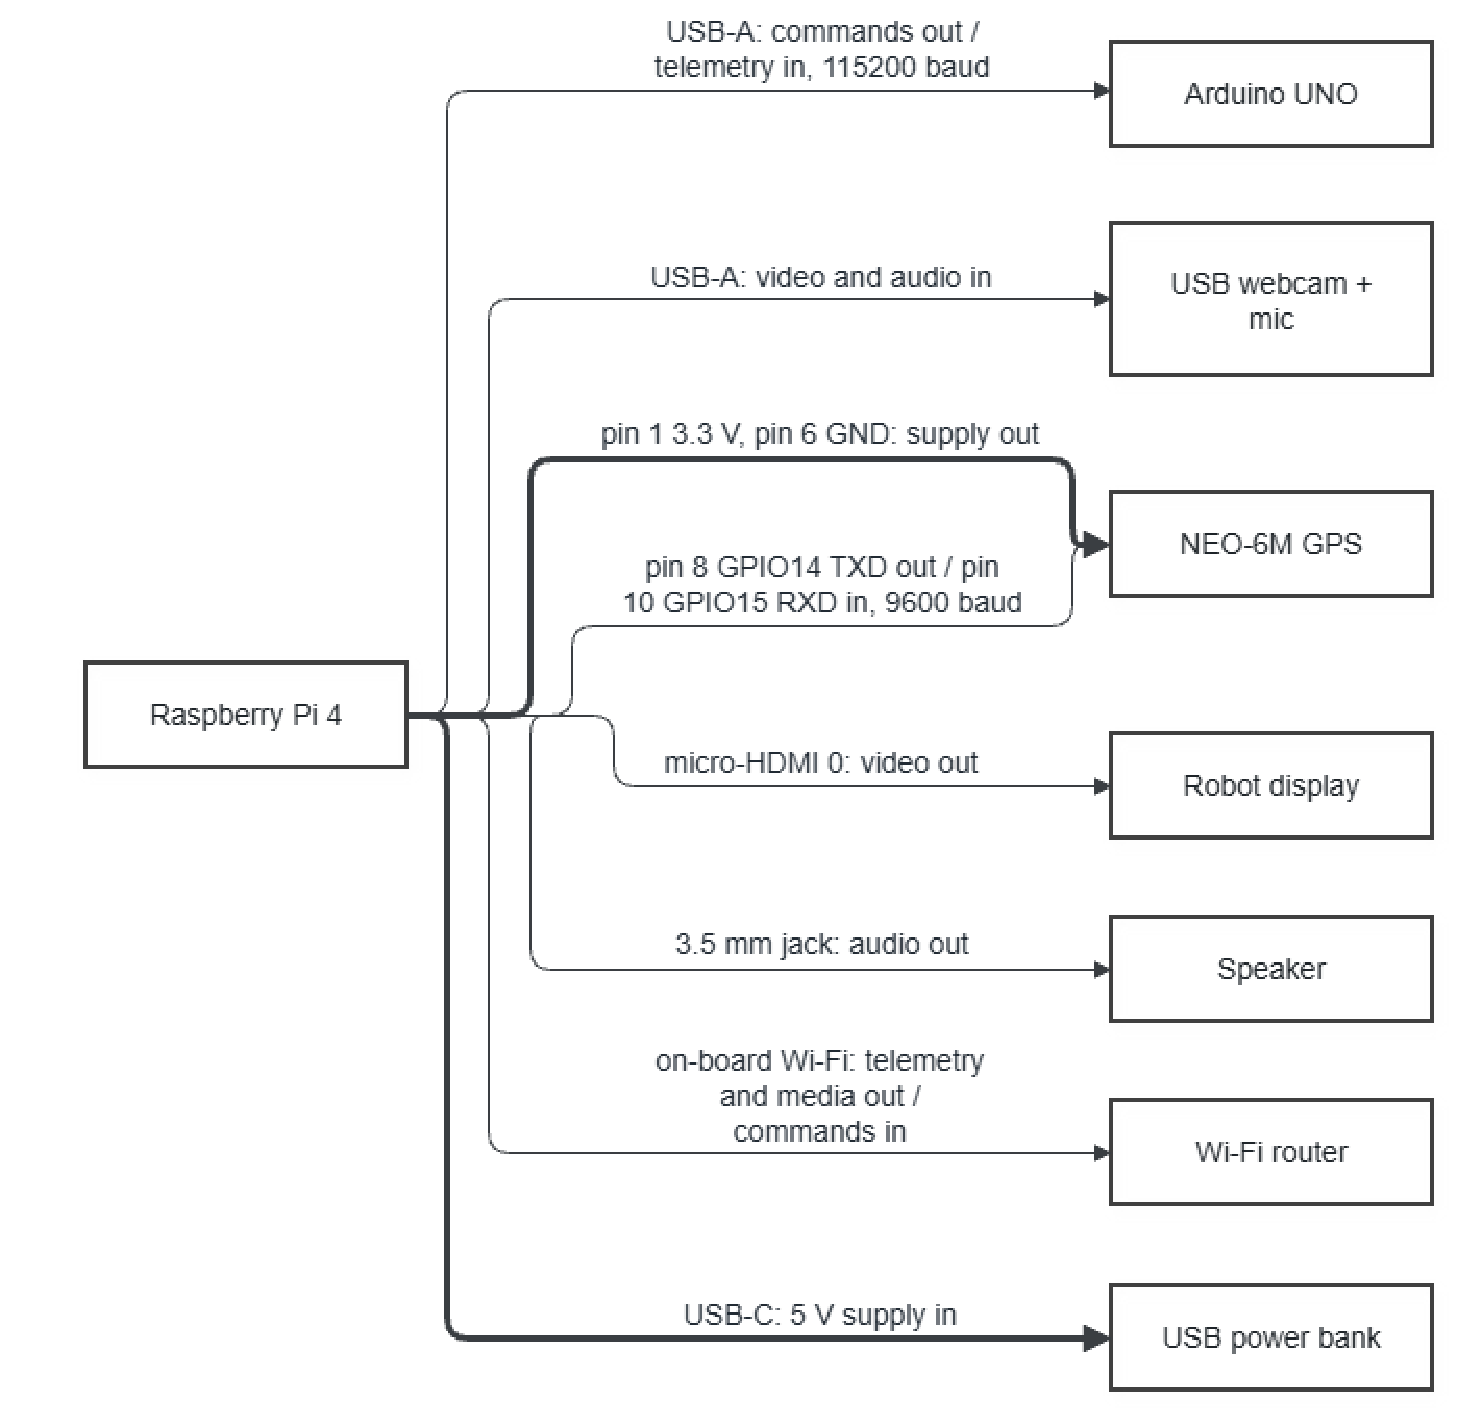
\includegraphics[width=0.9\textwidth]{fig05.pdf}
\caption{Raspberry Pi 4 port and GPIO diagram. Every line is drawn from the Pi outwards to the device it serves, so an arrowhead marks the connection and not the direction. Direction is given in the label instead, read from the Pi's side: "out" leaves the port or pin and "in" arrives at it. The thick lines carry power, and the Pi's own supply arrives on USB-C. Table~\ref{tab:pi-connections} gives the full connection list.}
\end{figure}

The GPS uses the Pi's primary UART with the serial login console disabled.

\section{Software Architecture}

The software is organised around the same tiers as the hardware in Section 3.3. This section gives its structure; Sections 3.5 to 3.10 describe each part in detail.

The software forms three layers, each written in the language that suits its hardware, over a shared module that the three Pi processes have in common (Table~\ref{tab:software-stack}). The three layers share no code and talk only through three defined interfaces: the serial command protocol between firmware and P1, the control WebSocket between the dashboard and P1, and WebRTC between the dashboard and P2. Each layer can therefore be built, tested and replaced on its own.

\begin{center}
\begin{longtable}{|p{2cm}|p{2.5cm}|p{1.8cm}|p{3.5cm}|p{3.5cm}|}
\caption{Software stack.}
\label{tab:software-stack} \\
\hline
\textbf{Layer} & \textbf{Runs on} & \textbf{Language} & \textbf{Main frameworks} & \textbf{Main modules} \\
\hline
\endfirsthead
\hline
\textbf{Layer} & \textbf{Runs on} & \textbf{Language} & \textbf{Main frameworks} & \textbf{Main modules} \\
\hline
\endhead
Firmware & Arduino UNO & C++ & Arduino core, no RTOS & scheduler, command\_parser, motors, servos, sensors, telemetry \\
\hline
Backend & Raspberry Pi 4 & Python 3, asyncio & FastAPI and uvicorn (P1, P2), aiortc and PyAV (P2), aiohttp (P3) & serial\_bridge, safety, websocket\_hub, gps\_reader, signaling, talkback, supervisor \\
\hline
Common & Raspberry Pi 4, inside P1, P2 and P3 & Python 3 & standard library only & protocol, config, access, logging\_setup, mock\_hardware \\
\hline
Frontend & Operator browser & TypeScript & React 19, Vite, Tailwind CSS, Leaflet with PMTiles & useControlSocket, useWebrtcVideo, useTalkback, DriveControl, EmergencyStop, MapPanel \\
\hline
\end{longtable}
\end{center}

On the Pi, systemd starts only the watchdog, which spawns the control and media servers as child processes (Figure 6). P1 holds every interface that can move the robot; P2 holds every media device; the Robot Screen kiosk runs in the desktop session.

\begin{diagramfig}
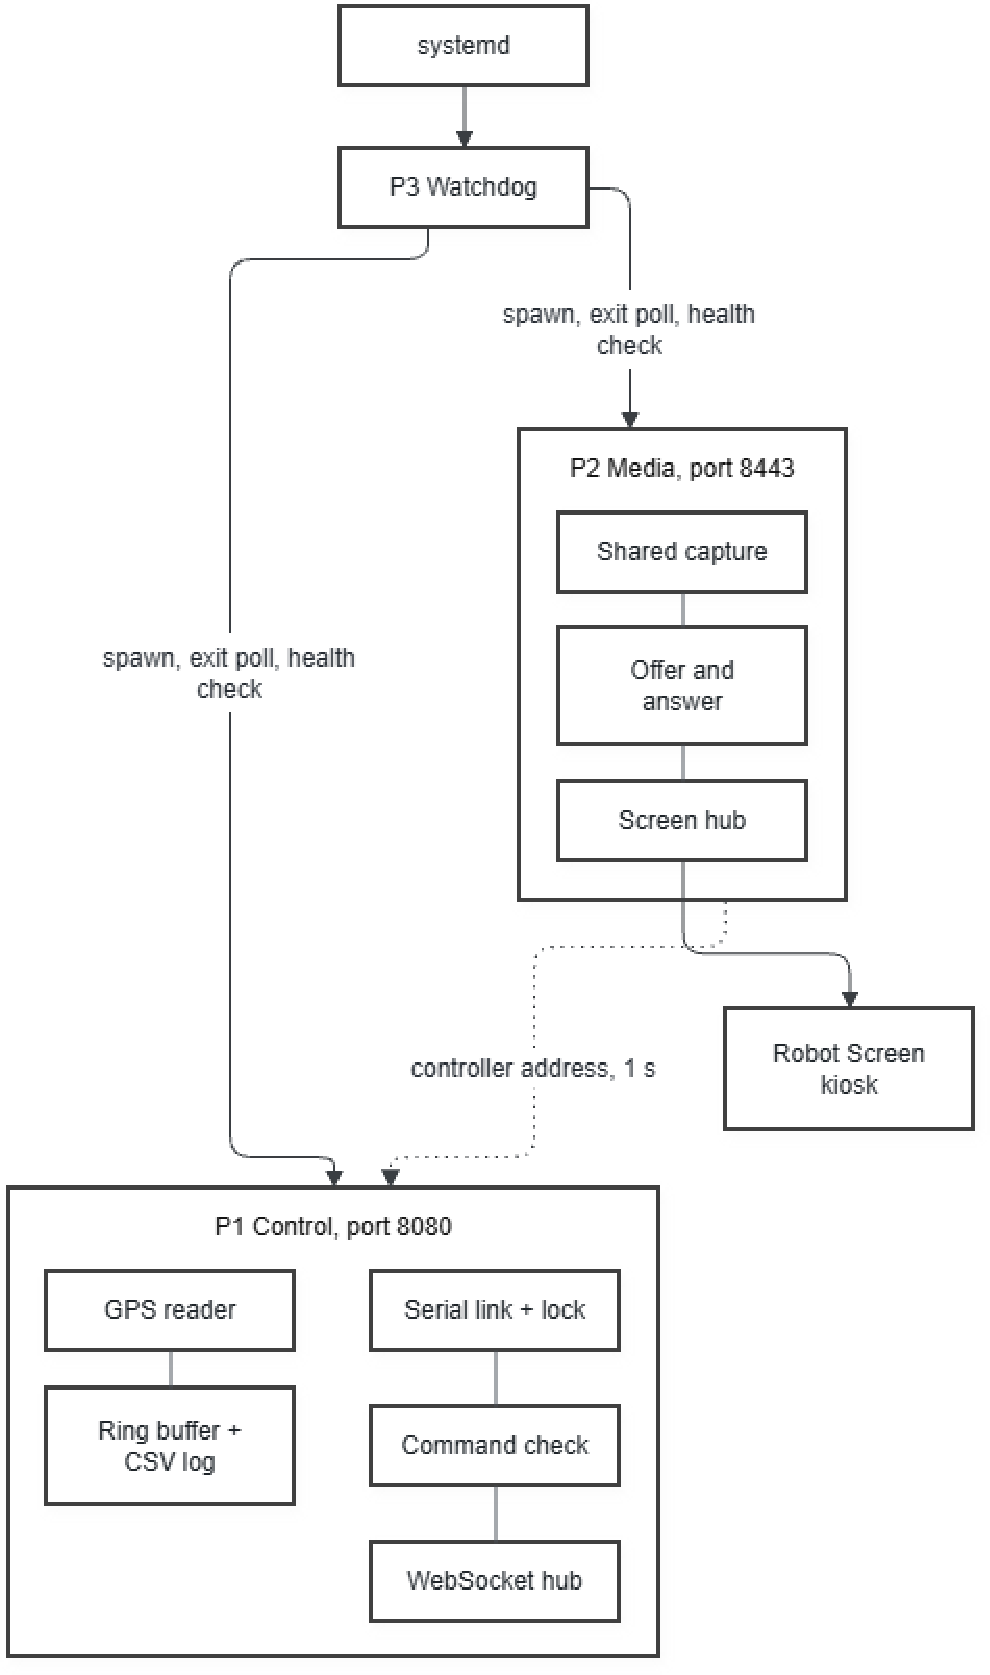
\includegraphics[width=0.9\textwidth]{fig06.pdf}
\caption{Raspberry Pi software architecture and process supervision.}
\end{diagramfig}

The dashboard is a single-page React application served by P1 (Figure 7). Its interface components hold no network code; they read state from, and send actions through, a small set of hooks. Each hook owns one connection to one server, so a lost media connection leaves the drive controls and telemetry working.

\begin{figure}[H]
\centering\footnotesize
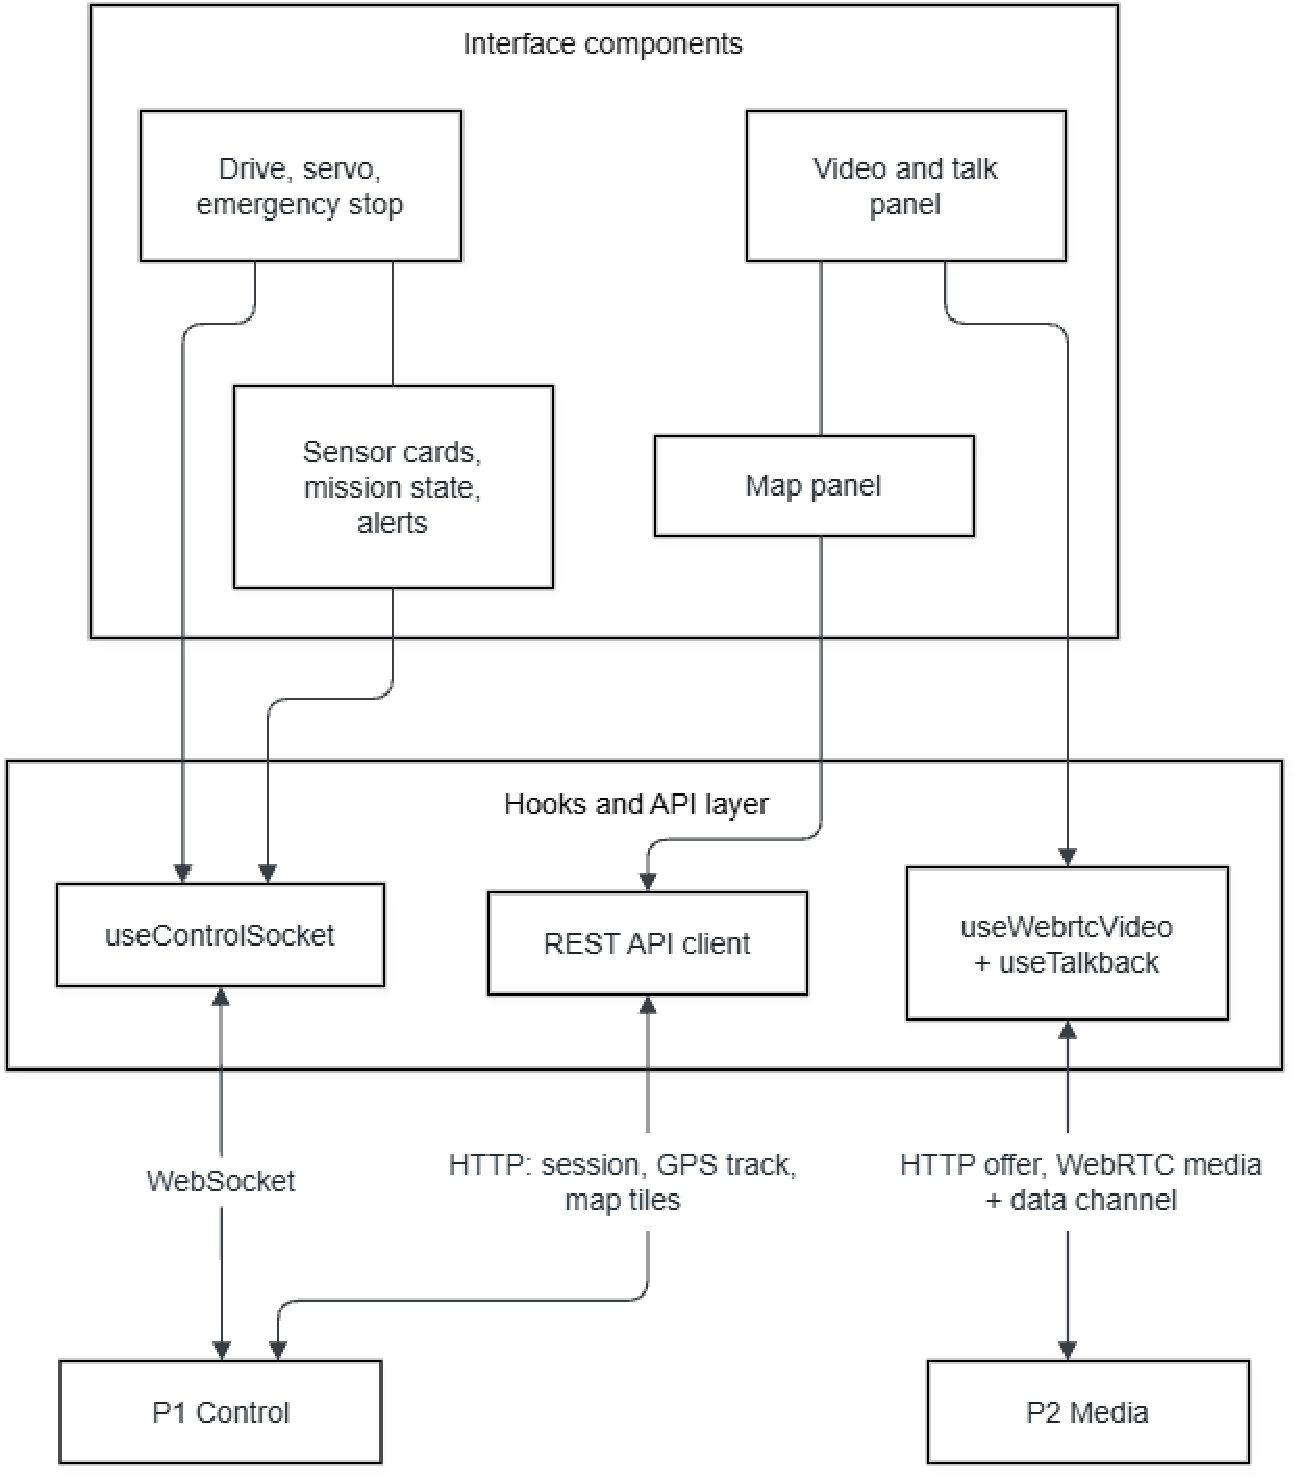
\includegraphics[width=0.55\textwidth]{fig07.pdf}

\vspace{6pt}
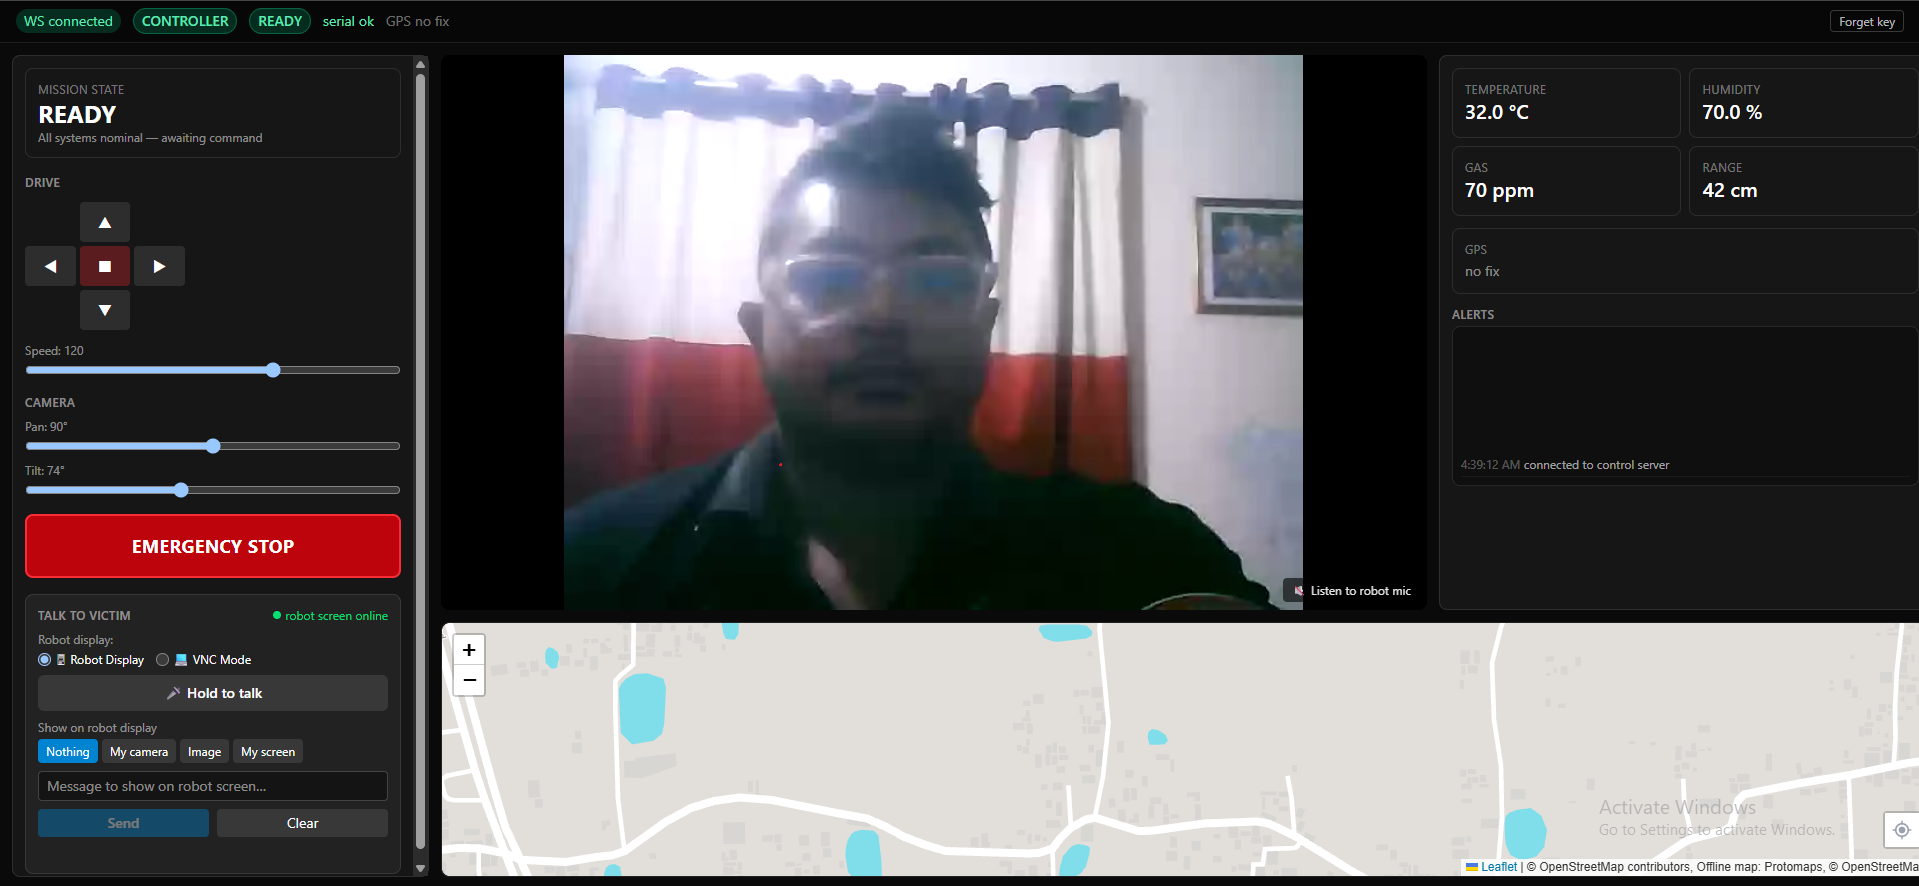
\includegraphics[width=0.95\textwidth]{fig07b.png}
\caption{Operator dashboard.}
\end{figure}

Each layer can also run without its hardware. A development mode (the MOCK\_HARDWARE setting) replaces the serial link with an in-process Arduino emulator that mirrors the firmware's framing, command validation, dead-man timer and telemetry cadence; replaces the GPS with a synthetic track; and replaces the camera and microphone with a synthetic video pattern and silence. The full control, telemetry, supervision and media stack therefore runs on a development machine with no robot attached, which is how the software is tested away from the hardware.

\section{Real-Time Firmware and Fail-Safe Control}

The firmware holds the authority to stop the robot, so it must stop the motors without help from the Pi or the network. The firmware defines five operating modes (Figure 8): BOOT, READY, ACTIVE, PANIC, and a reserved latched operator-stop mode, ESTOP. Motion is accepted only in READY and ACTIVE with no fault set; telemetry reports READY as 1, ACTIVE as 2 and all other modes (BOOT, PANIC and ESTOP) as 3.

\begin{figure}[H]
\centering\footnotesize
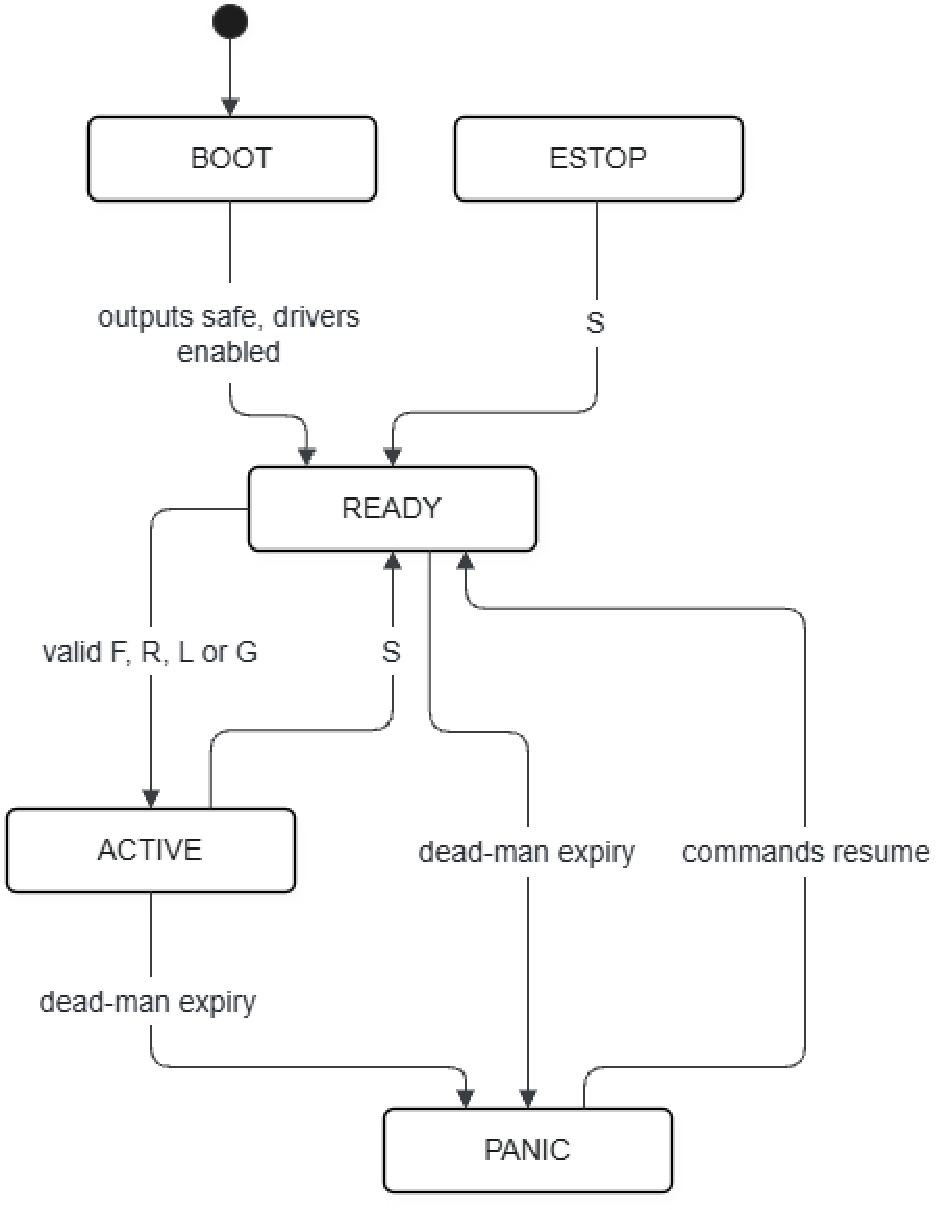
\includegraphics[height=15.3cm,keepaspectratio]{fig08.pdf}
\caption{Firmware operating modes. ESTOP is a reserved latched operator-stop state: it is defined in the firmware state machine and reported as 3, but is not entered in the current build, where the emergency stop is an ordinary S (Table~\ref{tab:stop-paths}).}
\end{figure}

\clearpage
\subsection{Task Scheduling and Command Validation}

A cooperative scheduler, rather than a pre-emptive RTOS on the ATmega328P \cite{pont2001}, runs the periodic tasks in Table~\ref{tab:firmware-tasks} from the main loop, with timing based on unsigned millisecond differences so that counter rollover does not break it. The command parser is polled on every loop pass and checks each command in four stages before it acts (Figure 9).

\begin{center}
\begin{longtable}{|p{3cm}|p{2.5cm}|p{6cm}|}
\caption{Firmware tasks.}
\label{tab:firmware-tasks} \\
\hline
\textbf{Task} & \textbf{Period} & \textbf{Work} \\
\hline
\endfirsthead
\hline
\textbf{Task} & \textbf{Period} & \textbf{Work} \\
\hline
\endhead
Motor service & 10 ms & Ramp PWM toward target by 15 units per tick \\
\hline
Safety supervisor & 10 ms & Dead-man check and fault recovery \\
\hline
Fast sensors & 50 ms & HC-SR04 range (25 ms echo timeout) \\
\hline
Slow sensors & 2000 ms & DHT11 and MQ-136 \\
\hline
Telemetry & 500 ms & One 8-field CSV line \\
\hline
Heartbeat & 1000 ms & Mode line and status LED toggle \\
\hline
\end{longtable}
\end{center}

The telemetry period (TELEMETRY\_PERIOD\_MS = 500 ms in \texttt{arduino/config.h}) and the ramp step (MOTOR\_RAMP\_STEP = 15) are the two firmware constants that bound the empirical stop-time distribution reported in Section 5.1.

\begin{figure}[H]
\centering\footnotesize
\makebox[\textwidth][c]{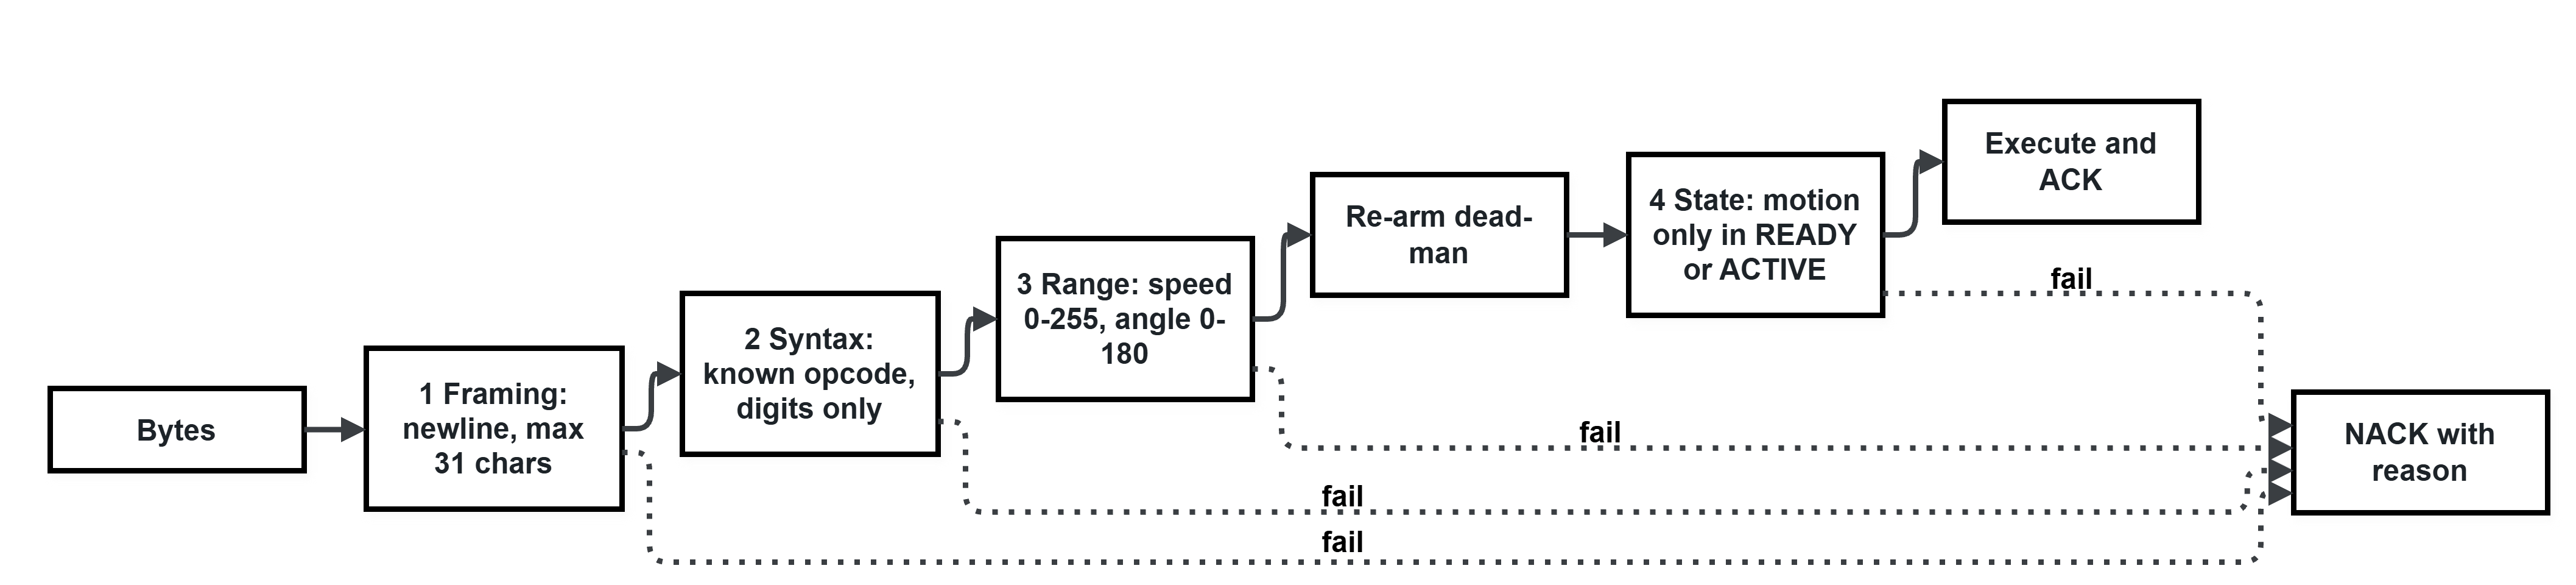
\includegraphics[width=1.15\textwidth]{fig09.png}}
\caption{Four-stage firmware-side command validation. The nine opcodes are F, R, L, G (speed), P, T (angle), S, H and ?.}
\end{figure}

\clearpage
The Pi control server applies a tighter safety cap before sending: speed is clamped to 0-180 (keeping the 14.8 V battery under the motor's \textasciitilde{}12 V rating) and angles to 0-180, and motion and servo commands whose sequence number is not higher than the last one from that client are rejected.

\subsection{Dead-Man Timer and Stop-Time Guarantee}

Every command that passes stages 1 to 3 re-arms the dead-man timer, including heartbeats; this dead-man (watchdog) pattern, in which loss of a periodic command forces the actuators to a safe state, behaves like the stop category 0 discussed in Section 2.3 \cite{iec60204}; it is a design choice here, not a claim of compliance. This is deliberately not limited to drive-type commands: pan, tilt and status-query commands pass the same three validation stages and therefore refresh the timer exactly as a drive or heartbeat command does (\texttt{command\_parser.cpp}'s \texttt{noteCommandReceived()} call sits after stage 3 and before the per-opcode state-machine gate, so it runs for every accepted opcode). The 2000 ms window is therefore measured from the last valid command of any kind, not specifically from the last drive command or the last heartbeat; an operator who is only panning the camera, with no drive command outstanding, keeps the dead-man armed without that being mistaken for continued motion. When the timer expires (the firmware's check is elapsed $\geq$ 2000 ms), the supervisor sets the PWM outputs to zero and pulls the shared enable line low at once, without ramping, and the firmware enters PANIC (Figure 10).

Two quantities follow from this and are kept apart throughout the paper: the stop time, when the motors lose drive, and the confirmation latency, when an observer outside the firmware can establish that they have. Only the first is a safety property.

The worst-case stop time after the last accepted command is:

\begin{equation}
t_{stop} \le T_{DM} + T_{S} + J
\end{equation}

where $T_{DM} = 2000$ ms is the dead-man window, $T_{S} = 10$ ms is the supervisor period, and $J$ is the longest single loop pass. $J$ is set by the two blocking sensor reads, the 25 ms HC-SR04 echo timeout and the DHT11 exchange whose 20 ms start pulse dominates it. Because the slow sensor period of 2000 ms is an exact multiple of the fast period of 50 ms (Table~\ref{tab:firmware-tasks}), the two reads coincide in one loop pass once every 2 s, so $J$ is about 50 ms rather than the cost of either read alone, and the bound is about 2060 ms. The bound is analytical. Section 5.1 supports it from the firmware side: on P1's clock the PANIC line, which the firmware emits in the same supervisor pass that removes drive, arrived within 2042 ms of the last command in 30 of 30 trials (Table 5.2b), a log-timed interval that includes serial transit and has a resolution of about 15 ms. It does not observe the wheels. The physical wheel-stop time, to be filmed at 240 fps (\texttt{tools/eval/record.py deadman\_physical}, E4), is [PENDING MEASUREMENT].

Confirmation latency is larger, by a margin that belongs to the reporting path and not to the stop. The firmware reports a trip on two paths over the one serial link. It emits a tagged PANIC line in the same supervisor pass that stops the motors, so that notice costs only serial transit; separately, the fw\_state field that encodes PANIC rides the periodic telemetry frame, which the firmware emits every 500 ms (Table~\ref{tab:firmware-tasks}) and which P1 rebroadcasts on its own 200 ms timer (Section 3.6.2). An observer that waits on fw\_state therefore learns of the trip up to 700 ms after the motors stop, and about 350 ms after it on average. The WebSocket probe reported in Section 5.1 (\texttt{tools/eval/wslatency.py}) waits on fw\_state, so its dead-man figures are confirmation latency along the slower of the two paths: an upper bound consistent with the stop-time bound above rather than a measurement of it. In the build evaluated here P1 writes the PANIC line to its log but does not forward it to the dashboard, so the operator display is driven by the 500 ms frame and the fast notice survives only as a log entry; Section 6.3 treats this as a limitation.

An ordinary stop command ramps the motors down instead:

\begin{equation}
t_{ramp} = \left\lceil \frac{u}{\Delta u} \right\rceil T_{M}
\end{equation}

where $u$ is the current PWM value, $\Delta u = 15$ is the ramp step and $T_{M} = 10$ ms is the motor service period; this gives 120 ms from the 180 cap and 170 ms from 255.

\begin{diagramfig}
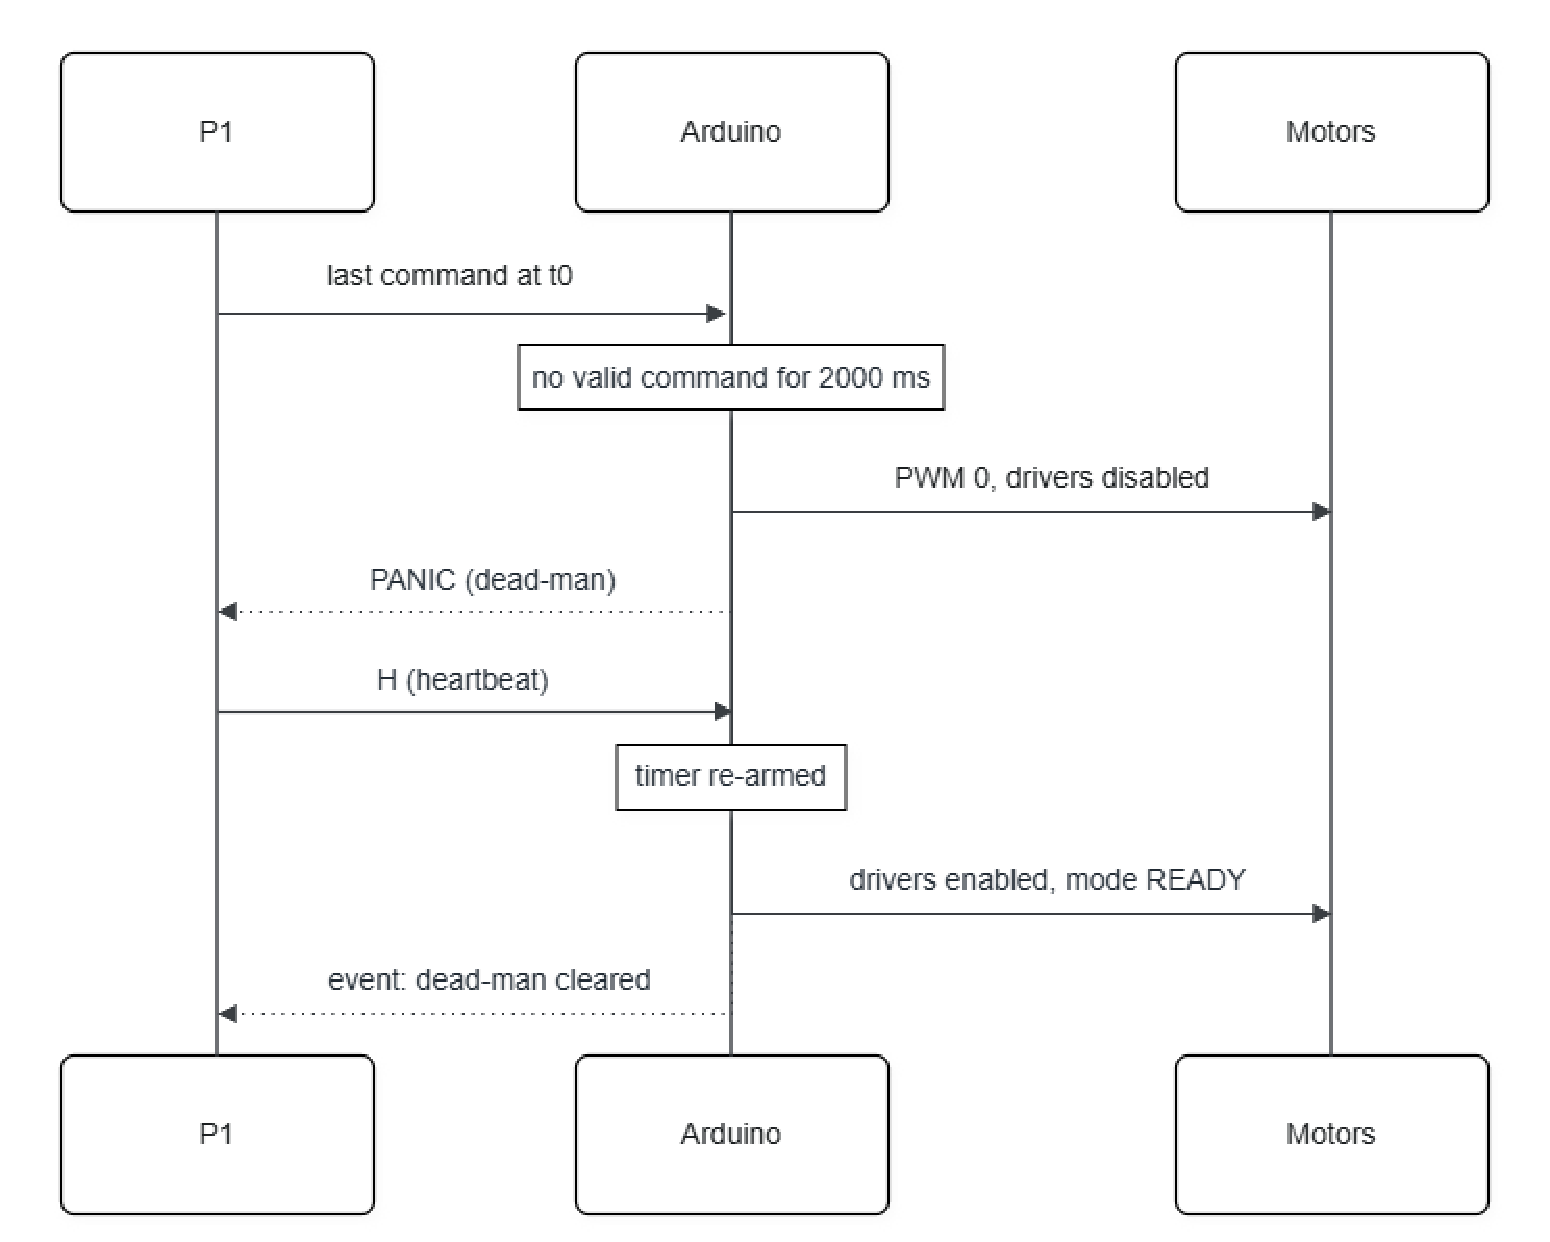
\includegraphics[width=0.9\textwidth]{fig10.pdf}
\caption{Dead-man trip and recovery.}
\end{diagramfig}

\subsection{Redundant Stop Paths}

Table~\ref{tab:stop-paths} lists every path that stops the motors. The firmware's only automatic stop is the dead-man; every other row is an operator action or a P1 action, and the firmware itself never stops the motors on a sensor reading. The MQ-136 gas sensor is advisory: its reading is published to the operator in telemetry and is not used to stop the motors.

\begin{center}
\begin{longtable}{|p{3.5cm}|p{2.5cm}|p{3cm}|p{3cm}|}
\caption{Stop paths.}
\label{tab:stop-paths} \\
\hline
\textbf{Trigger} & \textbf{Origin} & \textbf{Action} & \textbf{Bound} \\
\hline
\endfirsthead
\hline
\textbf{Trigger} & \textbf{Origin} & \textbf{Action} & \textbf{Bound} \\
\hline
\endhead
Drive key or button released & Dashboard via P1 & S, ramped stop & One network trip \\
\hline
Emergency stop button & Dashboard via P1 & S, sent without the sequence check & One network trip \\
\hline
Controller connection closes & P1 & S & On socket close \\
\hline
Another dashboard takes control & P1 & S & On takeover \\
\hline
P1 start-up & P1 & 3 x S, 200 ms apart & Before any other command \\
\hline
P1 shutdown & P1 & S & Before the port closes \\
\hline
Command flow stops & Firmware & PWM 0, drivers disabled & $t_{stop}$ above \\
\hline
\end{longtable}
\end{center}

\section{P1 Control Server and Telemetry}

The firmware stops the robot when commands cease, but it assumes that the commands it does receive come from one source and arrive in order. P1 provides that assumption and returns the robot's state to the operator. P1 owns the serial link, the GPS receiver and the control WebSocket.

\subsection{Safe Startup and Single-Writer Serial Link}

P1 takes an exclusive, non-blocking lock on a file in a memory-backed directory before it opens any hardware; the kernel releases the lock when the process exits for any reason. The serial port is then opened in exclusive mode, and one asynchronous lock serialises all writes. Figure 11 shows the start-up handshake.

\begin{diagramfig}
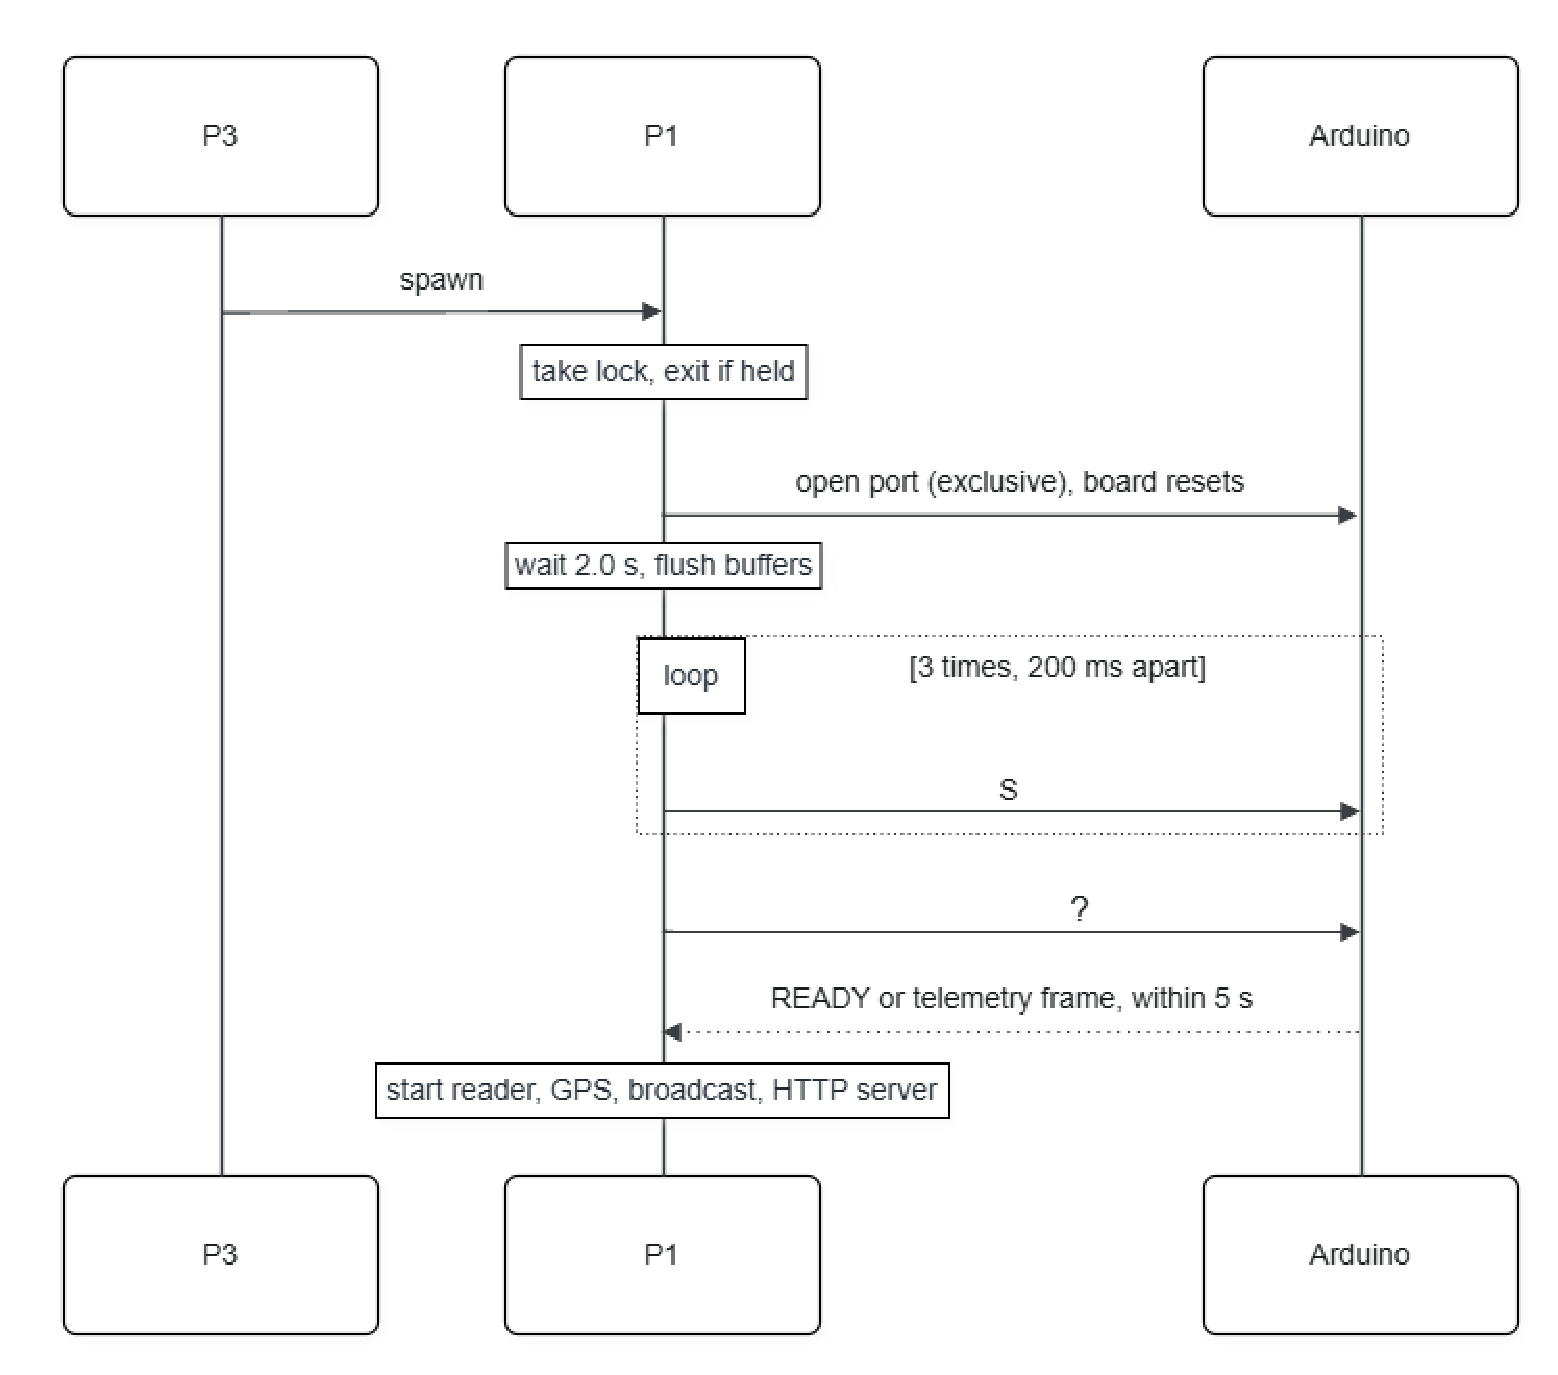
\includegraphics[width=0.9\textwidth]{fig11.pdf}
\caption{P1 start-up handshake. A timeout ends P1 with a handshake-failure exit code.}
\end{diagramfig}

\subsection{Telemetry Pipeline and Session Resume}

The firmware sends a frame every 500 ms; P1 broadcasts a snapshot of the latest valid frame every 200 ms on an absolute schedule, merged with GPS and link status (Figure 12). A frame is dropped if any field fails the checks in Table~\ref{tab:telemetry-fields}; there is no retransmission.

\begin{diagramfig}
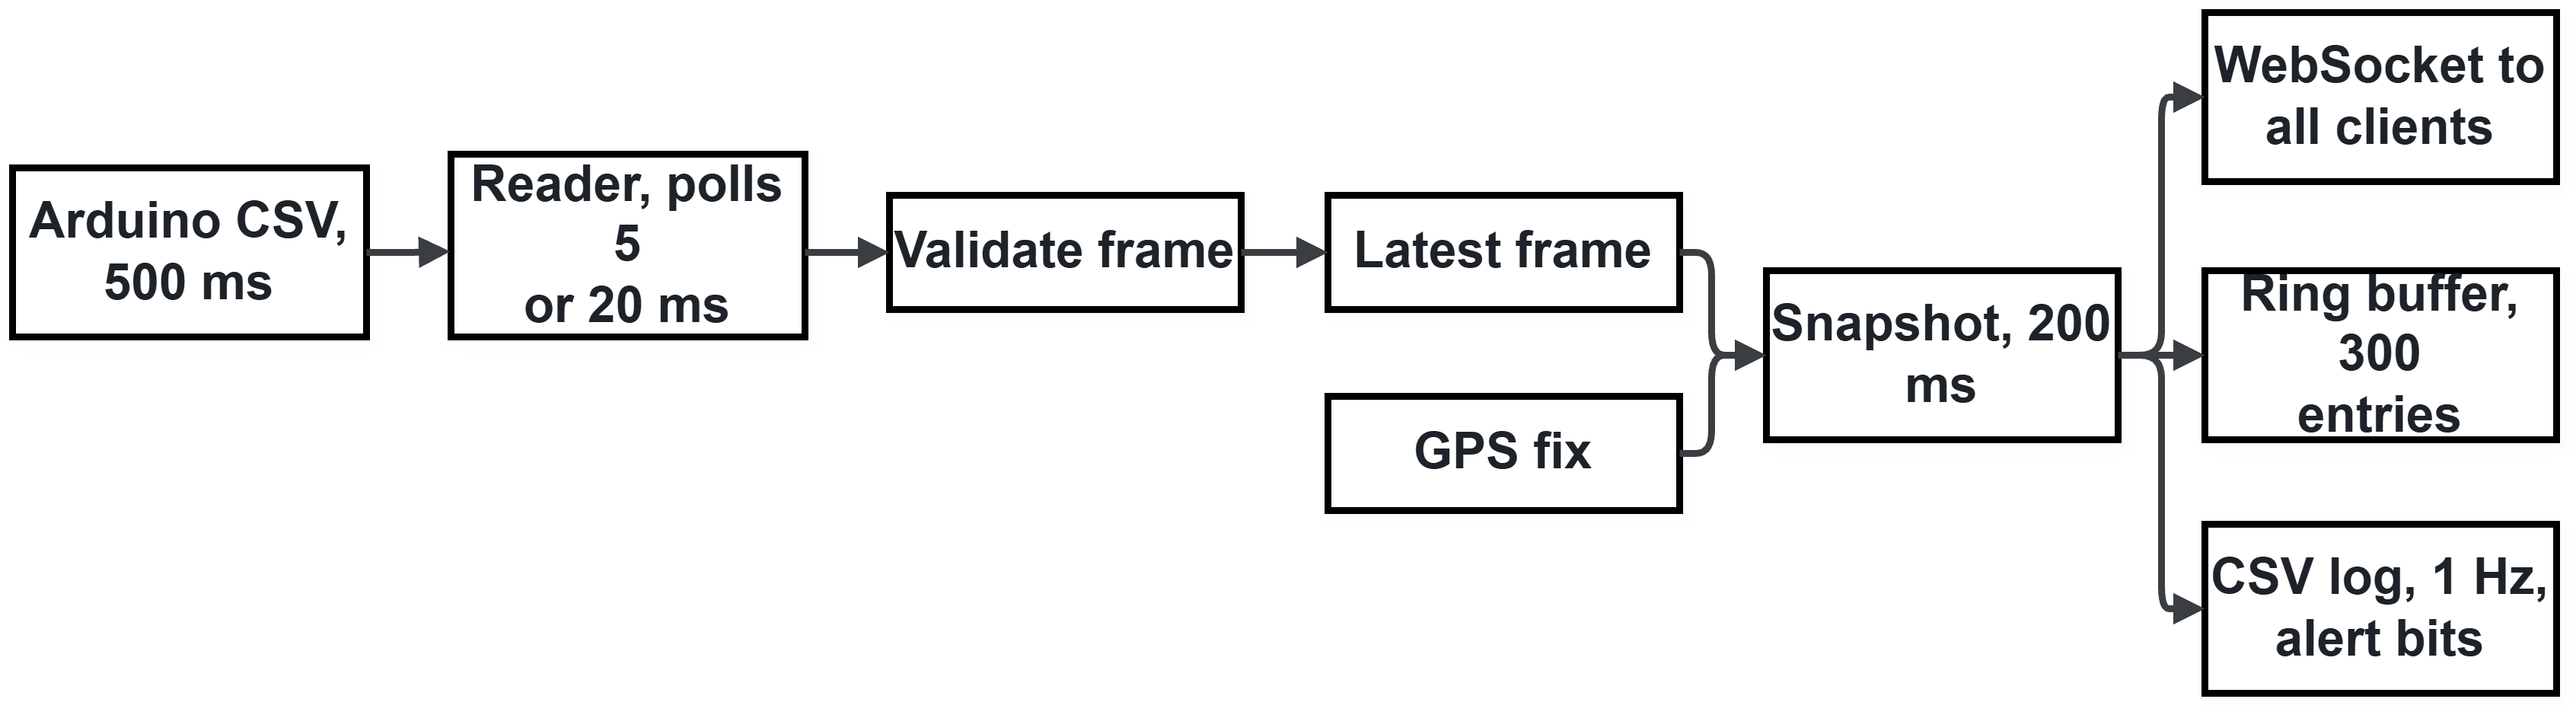
\includegraphics[width=0.9\textwidth]{fig12.png}
\caption{Telemetry pipeline.}
\end{diagramfig}

\begin{center}
\begin{longtable}{|p{3.5cm}|l|p{4cm}|}
\caption{Telemetry frame fields and accepted ranges (frame at most 80 characters).}
\label{tab:telemetry-fields} \\
\hline
\textbf{Field} & \textbf{Unit} & \textbf{Accepted range} \\
\hline
\endfirsthead
\hline
\textbf{Field} & \textbf{Unit} & \textbf{Accepted range} \\
\hline
\endhead
Temperature & degC & -40 to 125 \\
\hline
Humidity & \% & 0 to 100 \\
\hline
Gas & raw ADC & 0 to 10000 \\
\hline
Range & cm & 0 to 500 \\
\hline
Pan angle & deg & 0 to 180 \\
\hline
Tilt angle & deg & 0 to 180 \\
\hline
Firmware state & - & 1 to 3 \\
\hline
Uptime & ms & 0 to 2\textasciicircum{}32 - 1 \\
\hline
\end{longtable}
\end{center}

Because the P1 broadcast runs on an absolute schedule with period TELEMETRY\_PERIOD\_MS = 200 ms (\texttt{pi/common/protocol.py}), the control-plane latency probe in Section 4 jitters its send phase; a phase-locked sender produces a biased, deceptively tight distribution, as recorded in \texttt{tools/eval/README.md} and discussed in Section 6.4.

On reconnect, the dashboard sends the server timestamp of the last snapshot it received; P1 replies with every newer snapshot in the buffer and the size of any gap. The buffer depth and the gap are:

\begin{equation}
D = N \cdot T_{b} = 300 \times 200\ \text{ms} = 60\ \text{s}, \qquad g = \max(0,\ t_{oldest} - t_{last})
\end{equation}

where $N$ is the buffer size, $T_{b}$ the broadcast period, $t_{oldest}$ the oldest buffered timestamp and $t_{last}$ the client's last timestamp. The buffer is held in memory, so it does not survive a P1 restart.

\section{Fault Tolerance and Supervision}

Sections 3.5 and 3.6 make each tier fail into a stop; this section describes how failures are detected and how the system returns to service. Fault tolerance is layered (Figure 13). Each layer acts on its own, and a failure that passes every layer above ends at the firmware, which stops the motors.

\begin{diagramfig}
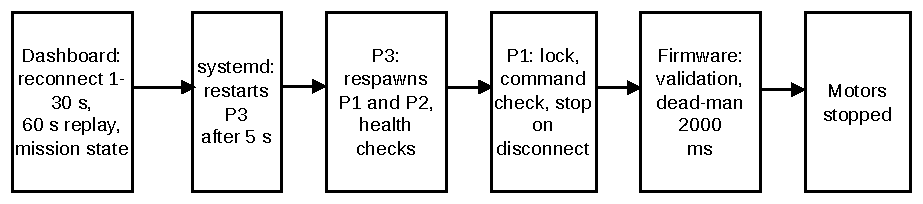
\includegraphics[width=0.9\textwidth]{fig13.pdf}
\caption{Layered fault tolerance, from the operator side down to the motors.}
\end{diagramfig}

\subsection{P3 Watchdog: Process Isolation and Supervision}

P3 is the only systemd service (restart on failure after 5 s); it spawns P1 and P2 as separate processes with no shared memory and supervises each one with the state machine in Figure 14. The only link between P1 and P2 is a once-per-second localhost query from P2 for the controller's address.

\begin{diagramfig}
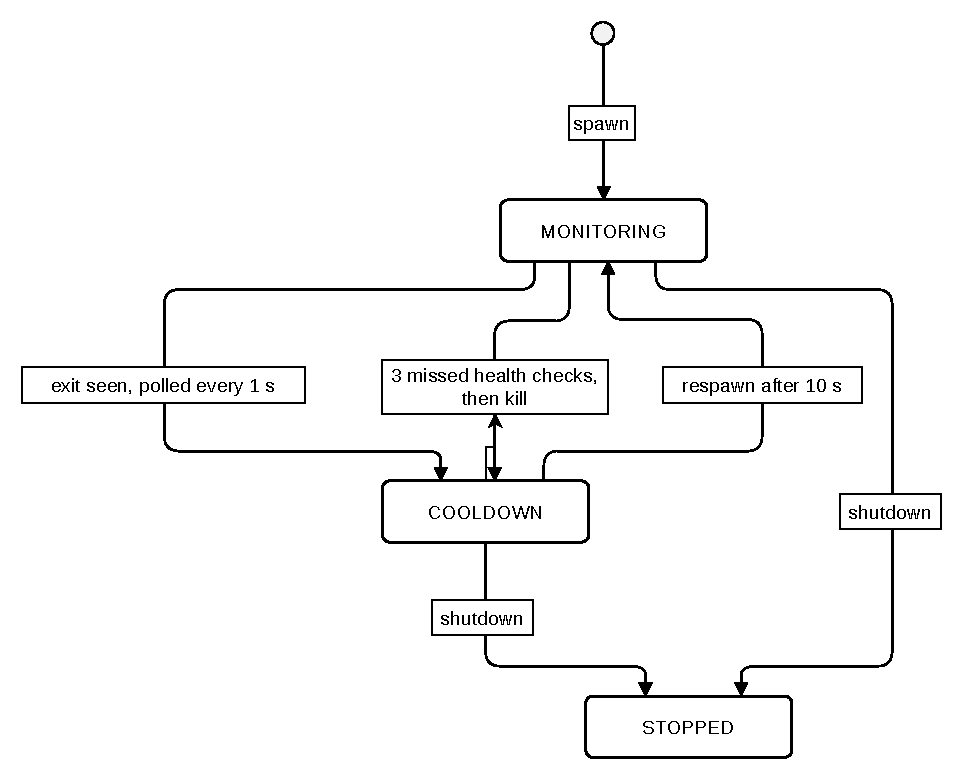
\includegraphics[width=0.9\textwidth,height=13cm,keepaspectratio]{fig14.pdf}
\caption{Per-process supervision. Health checks run every 10 s with a 5 s timeout.}
\end{diagramfig}

\subsection{Recovery Time Model and Graceful Degradation}

The time from a failure to a working process is:

\begin{equation}
T_{rec} = T_{det} + T_{p} + T_{c} + T_{init}
\end{equation}

where $T_{det}$ is the detection time (at most 1 s for a crash, at most $3 \times 10 + 5 = 35$ s for a hang), $T_{p} = 1$ s is the poll before cooldown, $T_{c} = 10$ s is the cooldown, and $T_{init}$ is start-up time, which for P1 is 2.0 s + 3 x 0.2 s plus up to 5 s for the handshake. A P1 crash therefore recovers in 14.6 s to 19.6 s plus interpreter start-up; the dashboard adds up to one reconnect back-off step. The constants in this model are validated against the fault-injection measurements of Section 5.4 (\texttt{tools/eval/faultinject.py}); the current campaign (10 trials each for F3 P1, F4 P2, F5 P3) is summarised in \texttt{tools/eval/results/summary.md}. Table~\ref{tab:failure-recovery} shows how each failure degrades the mission.

P1 reports why it exited through its process exit code, which the watchdog reads to decide how to react. A clean exit, or an exit because a healthy peer already holds the serial lock (code 0), draws no alarm: the watchdog simply waits out the cooldown rather than counting a crash. An unexpected lock error (code 1) or a failed Arduino handshake (code 2) is treated as a crash and respawned. An invalid configuration (code 3) is logged distinctly so that a persistent misconfiguration cannot drive a tight respawn loop. P2 uses the same configuration-invalid code.

\begin{center}
\begin{longtable}{|p{3cm}|p{2.5cm}|p{4cm}|p{4cm}|}
\caption{Failure effects and recovery.}
\label{tab:failure-recovery} \\
\hline
\textbf{Failure} & \textbf{Detected by} & \textbf{Effect} & \textbf{Recovery} \\
\hline
\endfirsthead
\hline
\textbf{Failure} & \textbf{Detected by} & \textbf{Effect} & \textbf{Recovery} \\
\hline
\endhead
Operator link lost & Dead-man; socket close & Robot stops; mission STOP & Reconnect with back-off, telemetry replay \\
\hline
P1 crash or hang & P3 & No control or telemetry; dead-man stops robot & Respawn; buffered history lost \\
\hline
P2 crash & P3 & Video and talk lost; control unaffected; mission DRIVING LIMITED & Respawn; operator retries video \\
\hline
Arduino link error & Serial read or write error & Serial flag false; mission STOP & Reads retried every 0.5 s; port reopened when P1 restarts \\
\hline
Camera fails to open & Media server & Synthetic test pattern sent & Next session \\
\hline
Microphone lost & Media server & Silence sent & Reopen tried every 2 s \\
\hline
GPS port error & P1 & No fix; GPS-lost alert bit set & Port reopened after 2 s \\
\hline
Robot Screen browser exits & Kiosk launcher & Victim screen blank & Relaunch after 3 s \\
\hline
P3 crash & systemd & P1 and P2 stop with it; dead-man stops robot & Restart after 5 s, then P1 and P2 respawn \\
\hline
\end{longtable}
\end{center}

Figure 15 shows how one failure, a Wi-Fi drop, passes through the tiers and how the system returns to service without operator action beyond reconnecting.

\begin{diagramfig}
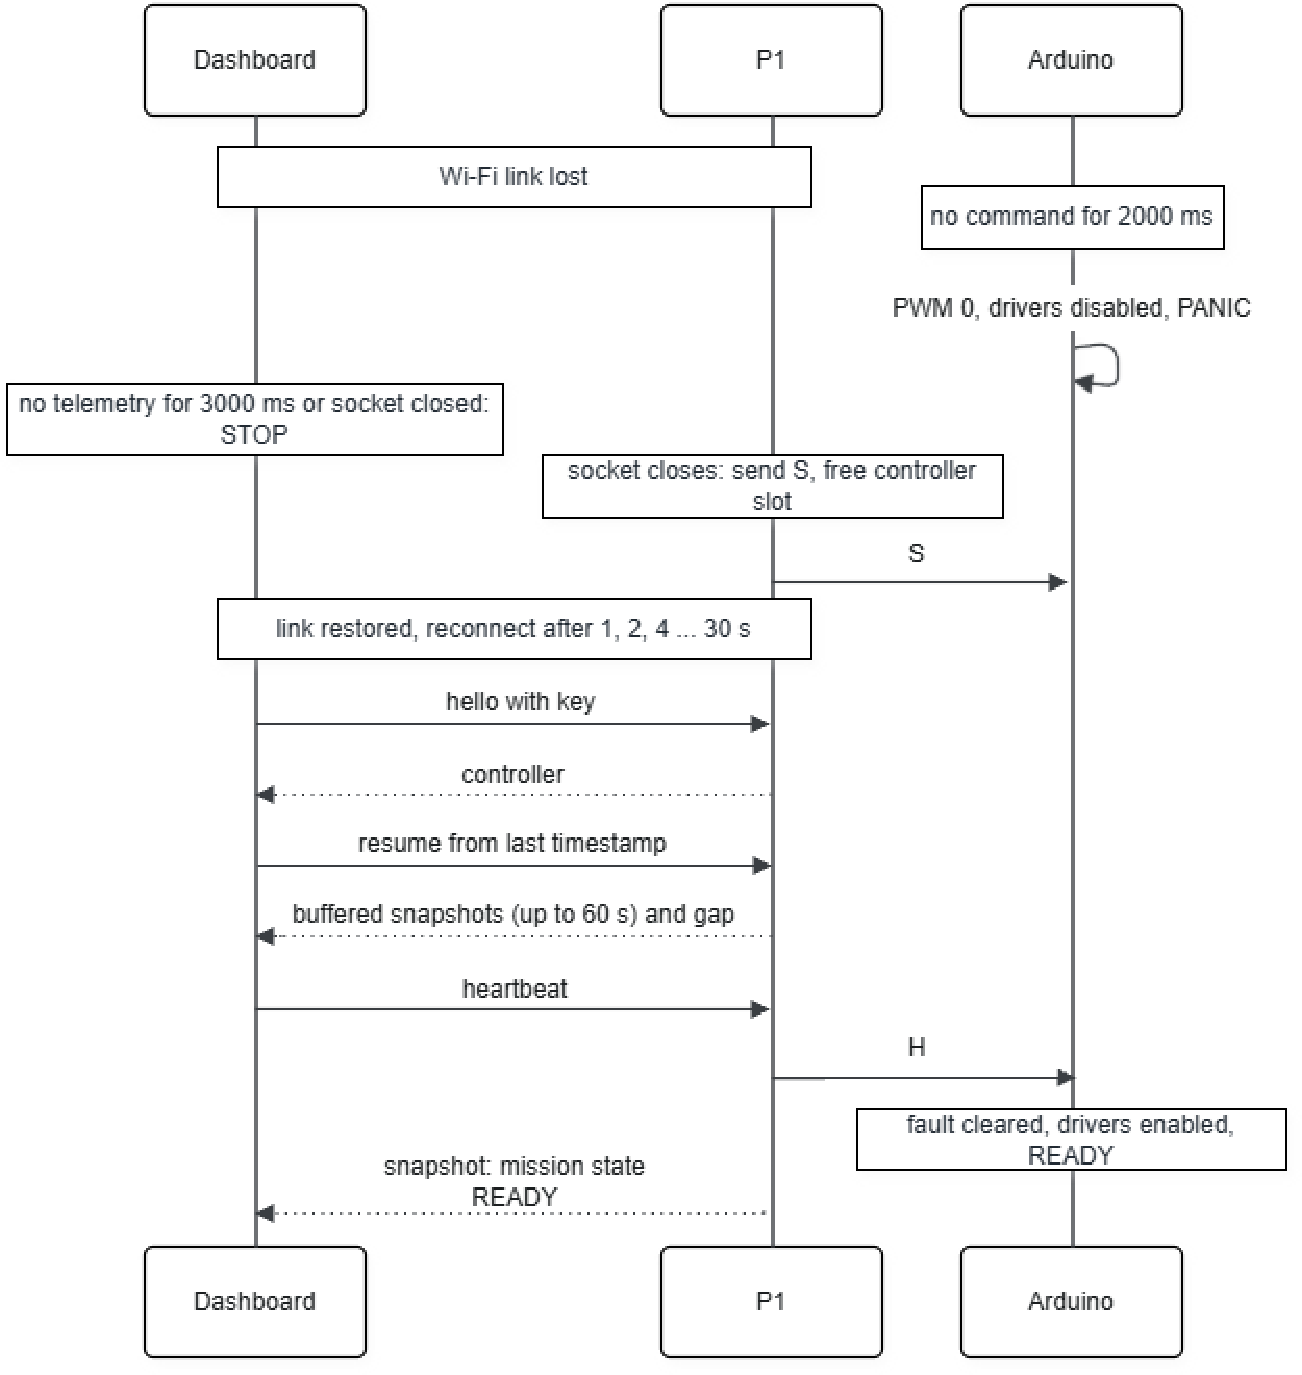
\includegraphics[width=0.9\textwidth]{fig15.pdf}
\caption{Failure chain for a Wi-Fi drop: stop, reconnect, replay, resume.}
\end{diagramfig}

\subsection{Mission State for Operator Awareness}

The dashboard reduces link and firmware status to one of four mission states, evaluated in the priority order of Table~\ref{tab:mission-state}.

\begin{center}
\begin{longtable}{|l|p{3cm}|p{7cm}|}
\caption{Mission state rules (first match wins).}
\label{tab:mission-state} \\
\hline
\textbf{Priority} & \textbf{State} & \textbf{Condition} \\
\hline
\endfirsthead
\hline
\textbf{Priority} & \textbf{State} & \textbf{Condition} \\
\hline
\endhead
1 & STOP & Control socket down, or serial link down, or no telemetry for more than 3000 ms \\
\hline
2 & DRIVING LIMITED & Video link down \\
\hline
3 & DRIVING & Firmware reports driving \\
\hline
4 & READY & Otherwise \\
\hline
\end{longtable}
\end{center}

\section{Access Control and Multi-Operator Arbitration}

Because any dashboard may reconnect after a failure (Section 3.7), the system must also decide which of several connected dashboards may drive. The decision is made once, in P1, and Section 3.9 reuses it for victim interaction. A dashboard becomes controller only by presenting the robot's controller key; all others are observers, whose commands, including stop, are rejected. The most recent dashboard with the right key takes the controller slot; the previous holder is demoted and the robot is stopped (Figure 16). P1 and P2 check the key in the same way (Table~\ref{tab:key-check}), and P2 grants talk only to a keyed session from the host P1 reports as controller.

\begin{diagramfig}
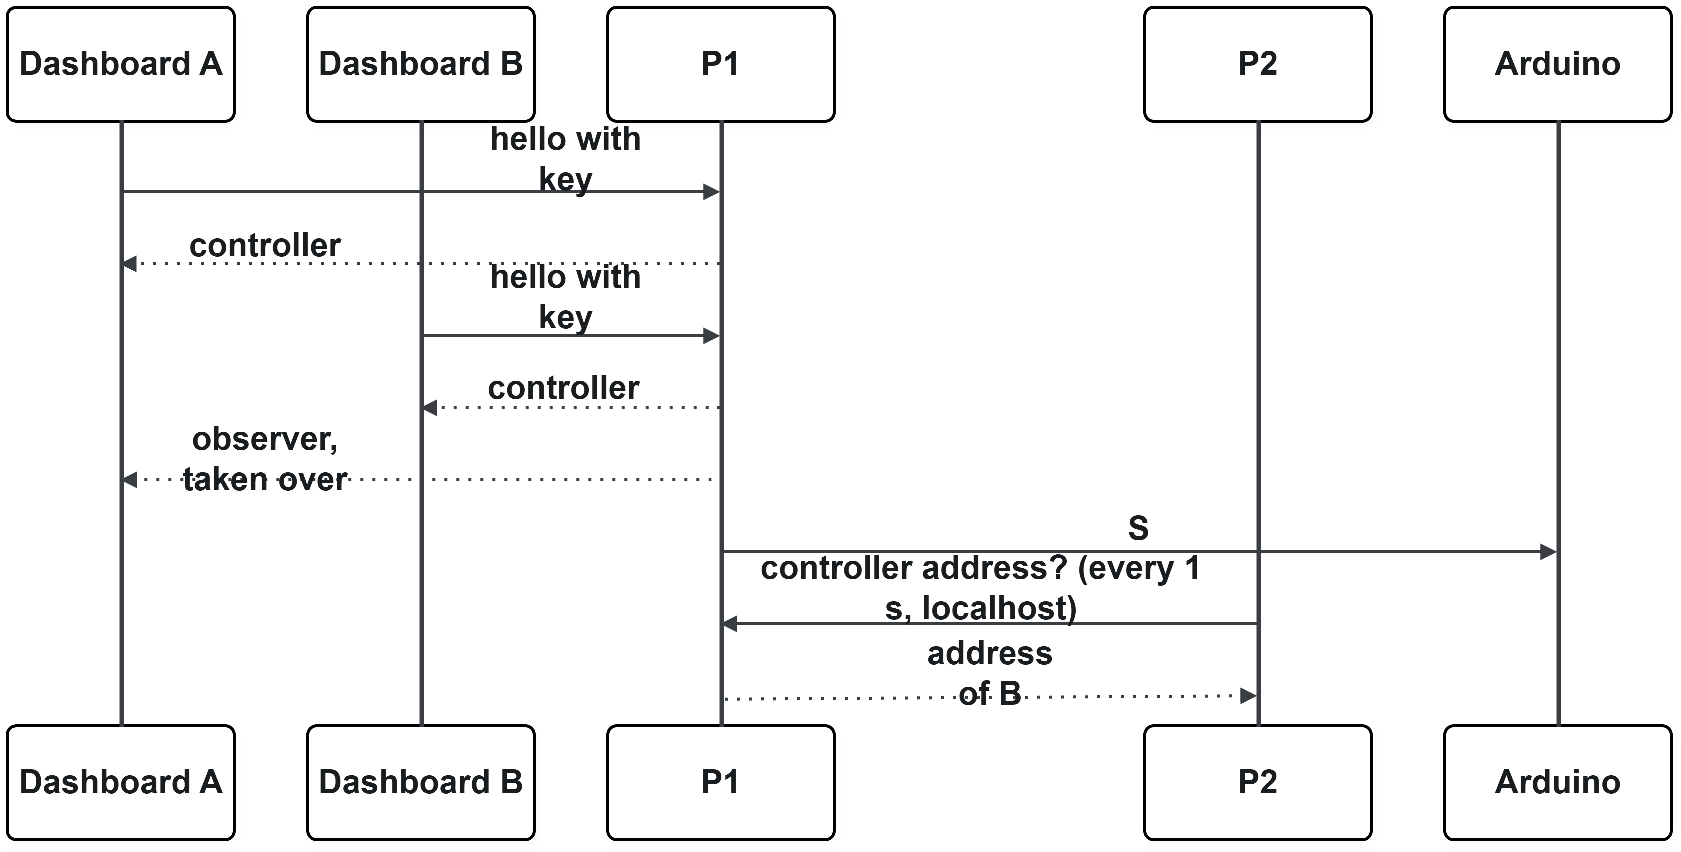
\includegraphics[width=0.9\textwidth]{fig16.pdf}
\caption{Controller takeover.}
\end{diagramfig}

\begin{center}
\begin{longtable}{|p{2.5cm}|p{5cm}|p{3cm}|}
\caption{Key check results.}
\label{tab:key-check} \\
\hline
\textbf{Result} & \textbf{Condition} & \textbf{Role} \\
\hline
\endfirsthead
\hline
\textbf{Result} & \textbf{Condition} & \textbf{Role} \\
\hline
\endhead
OK & Key matches (constant-time comparison) & Controller \\
\hline
No key & No key presented; not counted as a failure & Observer \\
\hline
Bad key & Wrong key; failure counted for that host & Observer \\
\hline
Locked & 5 failures within 300 s; host refused for 300 s, even with the right key & Observer \\
\hline
Disabled & No key configured on the robot & Observer for everyone \\
\hline
\end{longtable}
\end{center}

Failure counters are kept in memory per process. The dashboard discards a refused key so that reconnects do not add to the count. The key travels over plain HTTP and WebSocket. Both P1 and P2 accept requests from any origin (permissive CORS), because the dashboard may be served from the Pi, from a development server or from a content-delivery network, so its origin is not fixed; on the isolated local network this adds no exposure beyond the plain-HTTP key already noted.

\textbf{Threat model.} This design assumes a trusted local network at the staging point: operators are mutually authenticated with the robot by a shared controller key, and no on-path attacker is assumed on the Wi-Fi segment that carries both the plain-HTTP key and the WebSocket control plane. Transport confidentiality beyond WebRTC's own SRTP/DTLS, and defence against a Wi-Fi-adjacent adversary, are out of scope and are discussed in Section 6.3.

\section{Two-Way Victim Interaction}

With one controller established (Section 3.8), the same operator can see, hear and talk to the victim. This path must never delay a stop. The robot carries a display and speaker facing the victim, driven by a kiosk browser (the Robot Screen) on the Pi, and all communication between the operator and the victim runs through P2. Here ``P2'' names the media process (Section 3.4), not a peer-to-peer protocol.

aiortc was chosen over server-oriented WebRTC stacks such as GStreamer's webrtcbin, Janus and mediasoup because it integrates as a single Python process with the P2 asyncio event loop, reuses one PyAV capture across sessions, and needs no separate signalling server, following established use of WebRTC for low-latency teleoperation \cite{shi2025webrtc}. Human-subject interaction in this design, namely the Robot Screen used with role-played victims and the usability study with 8 to 12 operators (Section 5.8), is conducted under the ethics statement in Section 4.1.

Media is kept out of P1 because video encoding is the heaviest load on the Pi, and a stall or crash in a codec library must not delay a stop; P2 can also be restarted while P1 keeps driving (Table~\ref{tab:failure-recovery}). The only link between them is P2's once-per-second query for the controller's address (Section 3.7.1); P2 never sends anything to P1 or to the Arduino.

\subsection{The P2 Media Process}

P2 is a single Python process built on aiortc, a WebRTC implementation for asyncio, with PyAV (FFmpeg) for capture, decoding and encoding; every peer connection runs on one event loop (Figure 6).

\begin{itemize}
\item \textbf{Shared capture.} The webcam (V4L2) and the microphone (ALSA) can each be opened only once, so P2 opens each device on first use and fans its frames out to every session. Video is unbuffered, since a viewer needs only the newest frame; audio is buffered per session, since every audio frame matters. If the camera cannot be opened, the session receives a synthetic test pattern; if the microphone is missing or drops off USB, the session receives silence and P2 retries the device every 2 s.
\item \textbf{Per-session tracks.} Each dashboard session gets its own outbound video and audio track, and a private copy of every camera frame for its own encoder.
\end{itemize}

Each dashboard opens one peer connection to P2 that carries both directions at once: P2 sends the robot's camera and microphone to the operator, and the operator sends voice, video and text back over the same connection (Figure 17). Any number of dashboards may connect; all receive the robot's media, but only the controller can send to the Robot Screen. Table~\ref{tab:video-parameters} lists the video parameters.

\begin{diagramfig}
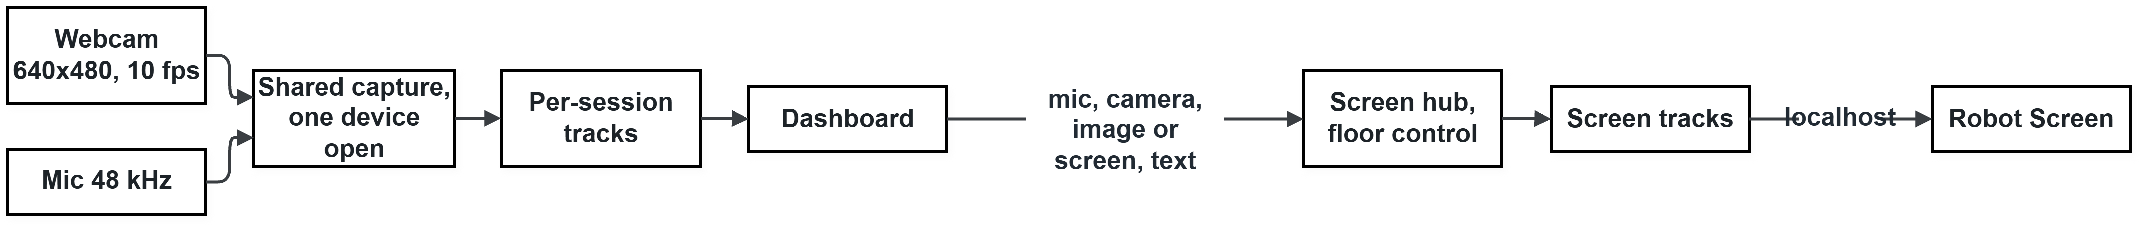
\includegraphics[width=1.0\textwidth]{fig17.pdf}
\caption{Two-way media path (WebRTC). Video is encoded per session as VP8 or H.264, as negotiated with the browser; each session gets its own copy of every camera frame.}
\end{diagramfig}

\begin{center}
\begin{longtable}{|p{3cm}|p{4.5cm}|p{4.5cm}|}
\caption{Video parameters.}
\label{tab:video-parameters} \\
\hline
\textbf{Parameter} & \textbf{Robot to operator} & \textbf{Operator to robot} \\
\hline
\endfirsthead
\hline
\textbf{Parameter} & \textbf{Robot to operator} & \textbf{Operator to robot} \\
\hline
\endhead
Source & USB webcam, V4L2 & Laptop camera, still image or shared screen \\
\hline
Resolution and rate & 640x480, 10 fps & Camera 640x480 at 10 fps; image 1024x576 at 2 fps; screen at 5 fps \\
\hline
Bitrate target & 500 kbps & Chosen by the browser \\
\hline
Codec & VP8 or H.264, negotiated per session & Decoded by P2, re-encoded for the Robot Screen \\
\hline
Encoders & One per dashboard session & One, for the Robot Screen connection \\
\hline
Source loss & Synthetic test pattern & Last frame repeated after 1 s; black frame when no operator video \\
\hline
\end{longtable}
\end{center}

\subsection{Signalling and Session Lifecycle}

The dashboard sends its SDP offer in one HTTP POST, together with its controller key if it has one, and the answer comes back in the HTTP response (Figure 18). There is no separate signalling server and no trickle ICE: P2 finishes gathering its candidates before it replies, so the answer is complete when it arrives. Because both peers are on the same local network, a direct host-to-host path is always available and no TURN relay is needed. The response also reports the key check result (Section 3.8), so the dashboard knows at once whether the session can talk or only watch.

\begin{diagramfig}
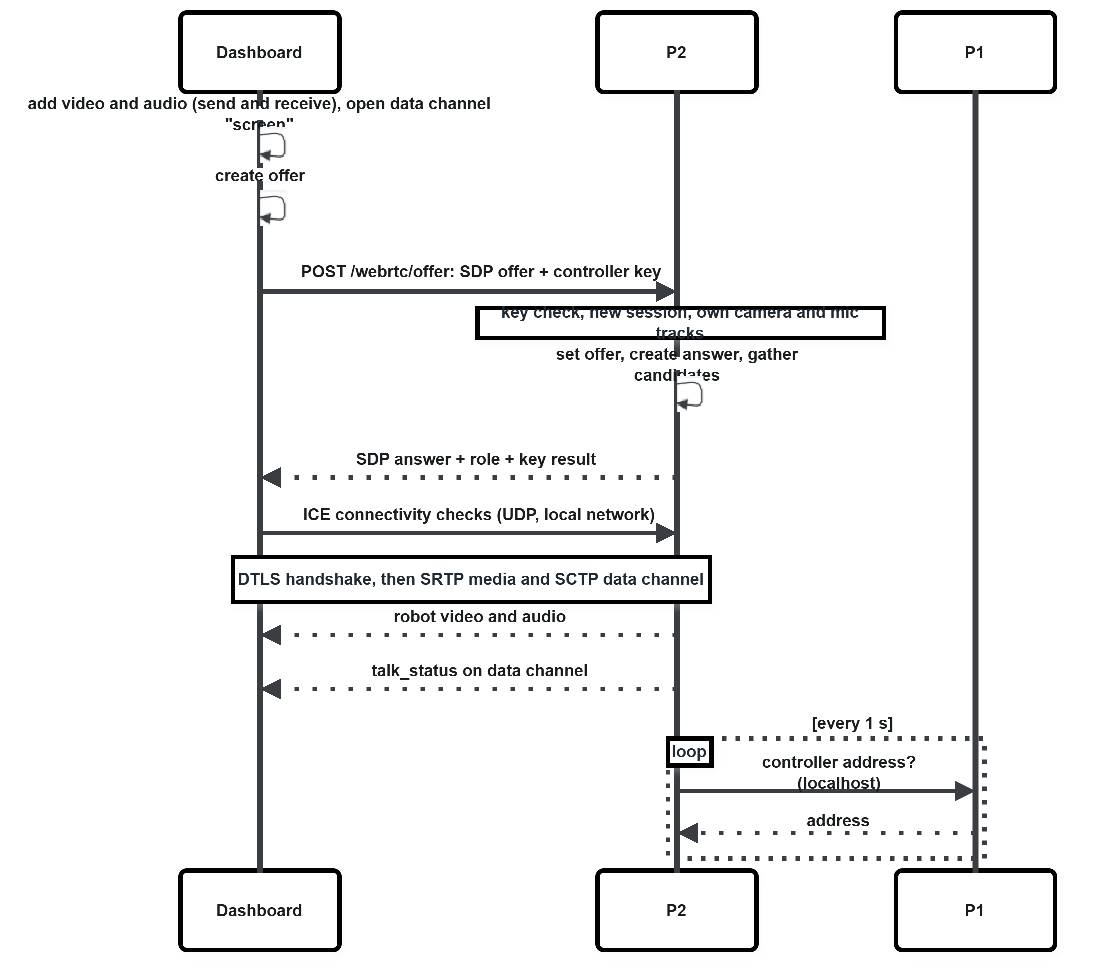
\includegraphics[width=\textwidth]{fig18.pdf}
\caption{WebRTC signalling and session set-up between a dashboard and P2.}
\end{diagramfig}

The dashboard offers its audio and video in both directions from the start, but sends nothing until the operator chooses to talk or show video; it then attaches the chosen source to the existing sender. Starting or stopping talk or video therefore never needs a second offer and answer.

When a connection fails or closes, P2 removes the session and releases the floor if the session held it; when no session is left, the camera and microphone are closed. P2 keeps no state that survives a restart, so reconnection is driven by the client. After video has connected once, a later loss is shown to the operator with a retry button rather than hidden by silent reconnects, so the operator knows that the video was interrupted.

Candidate gathering needs no help on this network. The dashboard creates its peer connection with no ICE servers configured, so both sides offer host candidates only, and the single segment of Section 3.2 makes a direct path available without STUN or a TURN relay. P1 does serve an ICE-configuration endpoint (GET /api/ice-config, rate limited to five requests per minute per client) for a deployment that would need STUN, but the dashboard does not read it in the local-network mode evaluated here. An internet-overlay mode, in which the robot would be reached through a relay and the same endpoint would also issue a TURN server, is provided for in the configuration (the ENABLE\_OVERLAY setting in the watchdog environment) but is not implemented or evaluated in this work; the turn\_status field carried in each telemetry snapshot therefore reports unavailable throughout.

\subsection{Data Channel Protocol}

Each dashboard connection carries one reliable, ordered data channel named ``screen'' over the same DTLS connection as the media. It carries short JSON messages for control of the Robot Screen (Table~\ref{tab:data-channel}); media and drive commands never travel on it. P2 validates every message: malformed messages are dropped, and messages from a session that is not the controller are refused with a view-only reply.

\begin{center}
\begin{longtable}{|p{3cm}|p{3.5cm}|p{5cm}|}
\caption{Data channel messages.}
\label{tab:data-channel} \\
\hline
\textbf{Message} & \textbf{Direction} & \textbf{Purpose} \\
\hline
\endfirsthead
\hline
\textbf{Message} & \textbf{Direction} & \textbf{Purpose} \\
\hline
\endhead
media\_state & Dashboard to P2 to Robot Screen & Operator is talking or not; which video source is shown \\
\hline
screen\_text & Dashboard to P2 to Robot Screen & Text message for the victim (at most 280 characters, with a timestamp) \\
\hline
screen\_clear & Dashboard to P2 to Robot Screen & Remove the text from the screen \\
\hline
floor\_release & Dashboard to P2 & Give up the Robot Screen \\
\hline
display\_mode & Dashboard to P2 & Switch the robot display between the kiosk and the Pi desktop \\
\hline
talk\_status & P2 to dashboard & Screen online, floor state (free, you, other), display mode, can control \\
\hline
screen\_state & P2 to Robot Screen & Whether an operator is present, talking or showing video \\
\hline
screen\_ack & Robot Screen to P2 to dashboard & The text with this timestamp is now shown \\
\hline
floor\_denied, view\_only & P2 to dashboard & Request refused: another operator holds the screen, or no controller key \\
\hline
\end{longtable}
\end{center}

The acknowledgement closes the loop for text: the dashboard marks a message as delivered only when the Robot Screen confirms it, not when it was sent. P2 sends talk\_status to every dashboard whenever the floor, the controller or the screen connection changes, so all operators see the same state.

\subsection{Operator-to-Robot Relay and Floor Control}

The operator's media does not go from the dashboard to the Robot Screen directly. The kiosk browser connects only to P2, over localhost, and P2 relays the operator's media to it. Floor control and the controller check are therefore enforced in one place, and no remote host can reach the victim's screen or speaker, since the screen endpoint refuses any address other than localhost. The kiosk also keeps one long-lived connection that does not change when operators connect, disconnect or take over.

The cost is one decode and one re-encode on the Pi. The Robot Screen connection has two fixed outbound tracks that always read from the current floor holder: the video track sends the holder's newest frame, repeating the last one after 1 s without a new frame and sending black when there is no operator video; the audio track re-encodes the holder's voice as 48 kHz mono, 60 ms Opus packets (Section 3.9.5), and sends silence otherwise. Because these tracks never change, talking, switching video sources and handing over the floor need no renegotiation.

Only one session may hold the Robot Screen at a time (Figure 19). Talking follows driving: P2 accepts talk, video and text only from a session that presented the controller key and comes from the address P1 reports as its controller (Section 3.8, Figure 16). A takeover therefore moves the talk path to the new driver within about one second. On release, P2 drops any queued operator media, clears the text and tells the screen that no operator is present.

\begin{diagramfig}
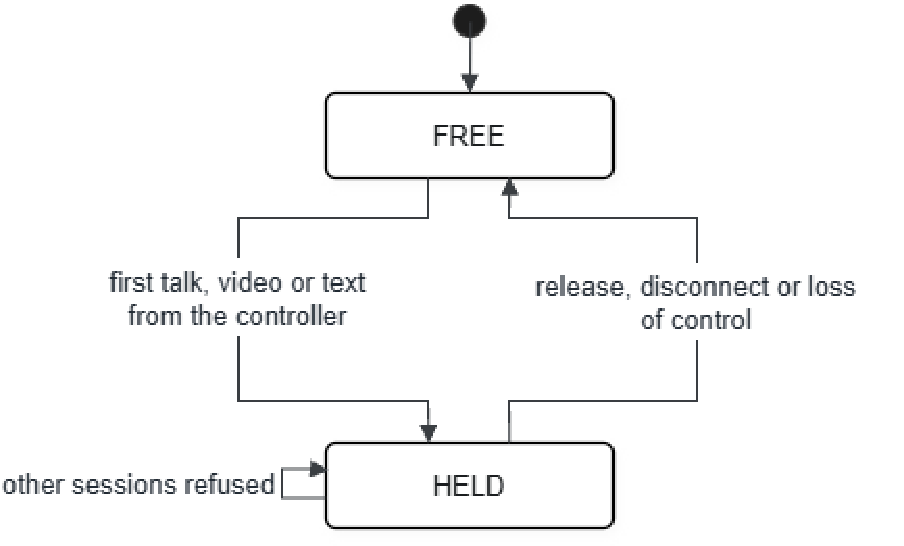
\includegraphics[width=0.9\textwidth]{fig19.pdf}
\caption{Robot Screen floor control. A release clears the screen text and media.}
\end{diagramfig}

\subsection{Low-Latency Audio on a Constrained CPU}

P2 encodes its own 60 ms Opus packets in both directions instead of the usual 20 ms \cite{valin2012}, which cuts the packet rate from 50 to 16.7 packets/s and the per-packet work on the event loop to a third. It captures the microphone through a shared ALSA device with a fixed period of 960 frames (20 ms), which gives 50 reads/s against about 511 reads/s for the device's smallest period of 94 frames (Table~\ref{tab:audio-parameters}).

\begin{center}
\begin{longtable}{|p{3cm}|p{4.5cm}|p{4.5cm}|}
\caption{Audio parameters.}
\label{tab:audio-parameters} \\
\hline
\textbf{Parameter} & \textbf{Robot to operator} & \textbf{Operator to robot} \\
\hline
\endfirsthead
\hline
\textbf{Parameter} & \textbf{Robot to operator} & \textbf{Operator to robot} \\
\hline
\endhead
Format & 48 kHz, mono, 16-bit & 48 kHz, mono, 16-bit \\
\hline
Codec & Opus, voice mode, 32 kbps & Opus, voice mode, 32 kbps \\
\hline
Packet length & 60 ms & 60 ms \\
\hline
Capture period and buffer & 960 frames (20 ms), 7680 frames (160 ms) & - \\
\hline
Buffering & One queue per session & Inbound queue of 10 frames (about 200 ms); 120 ms start cushion; 400 ms cap \\
\hline
Lateness & Paced by the device & Clock reset when more than 100 ms late, no catch-up burst \\
\hline
Source loss & Silence, reopen every 2 s & Silence until the cushion refills \\
\hline
\end{longtable}
\end{center}

\section{GPS Localisation and Offline Mapping}

The operator also needs to know where the robot is, both to guide it and to report the victim's position to the rescue team, without depending on the internet. P1 reads NMEA sentences from the NEO-6M receiver (\cite{ublox_neo6}; nominal accuracy 2.5 m CEP) on a separate thread, merges the latest fix into each telemetry snapshot (Section 3.6.2) and adds a track point only when the latest fix lies at least 10 m from the previous track point, which is intended to keep drift around a stopped robot out of the track (Figure 20). The filter compares positions held to six decimal places (about 0.1 m); the telemetry log, by contrast, records them to four (a grid of about 11 m by 10 m at the test latitude). The 10 m threshold lies above the receiver's nominal 2.5 m CEP, which the manufacturer specifies for 24 h static operation with strong signals \cite{ublox_neo6}, but not above the drift measured for this unit in the field: over 6888 logged fixes of a stationary robot with a mean of 4.8 satellites, about half lay more than 10 m from their centroid (CEP50 8.9 m and CEP95 30.5 m at the four-decimal logging resolution, \texttt{tools/eval/results/gps\_static.csv}), and in a later session in which the robot was not driven the filter added 130 track points (Section 5.6). The filter therefore reduces, but does not prevent, spurious track points under weak-signal conditions. Distance uses the equirectangular approximation:

\begin{equation}
d = R \sqrt{(\Delta\varphi)^2 + (\Delta\lambda \cos\bar{\varphi})^2}
\end{equation}

where $R = 6371000$ m, $\Delta\varphi$ and $\Delta\lambda$ are the latitude and longitude differences in radians, and $\bar{\varphi}$ is their mean latitude.

At the scales of these trials (under 2 km), the error of this approximation against the haversine formula stays below 0.01 mm at the trial latitude (computed over all bearings; 0.0036 mm at a 2 km baseline), which is negligible beside both the 10 m track filter and the metre-scale scatter of the receiver's fixes, while saving two trigonometric evaluations per update.

\begin{diagramfig}
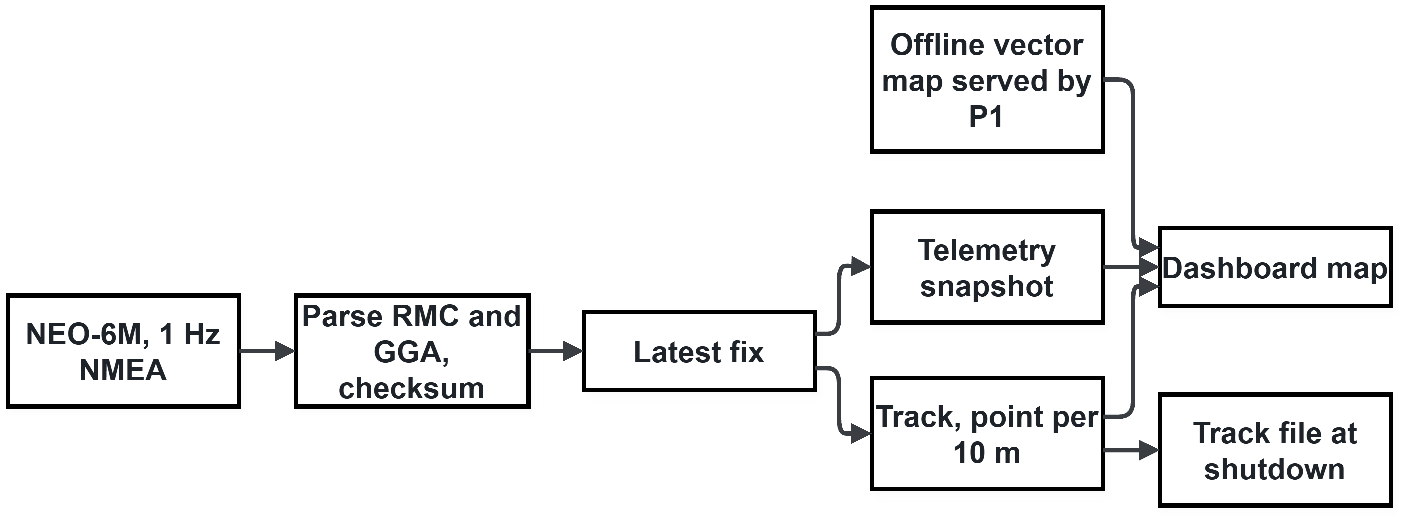
\includegraphics[width=0.9\textwidth]{fig20.pdf}
\caption{GPS and map data flow. Online map tiles, when reachable, show outside the offline map area.}
\end{diagramfig}
